\begin{figure*}
  \setlength\tabcolsep{\figstampcolsep}
  \begin{tabular}{l l l l l }
& &\multicolumn{2}{c}{\it Southeast group} \\
    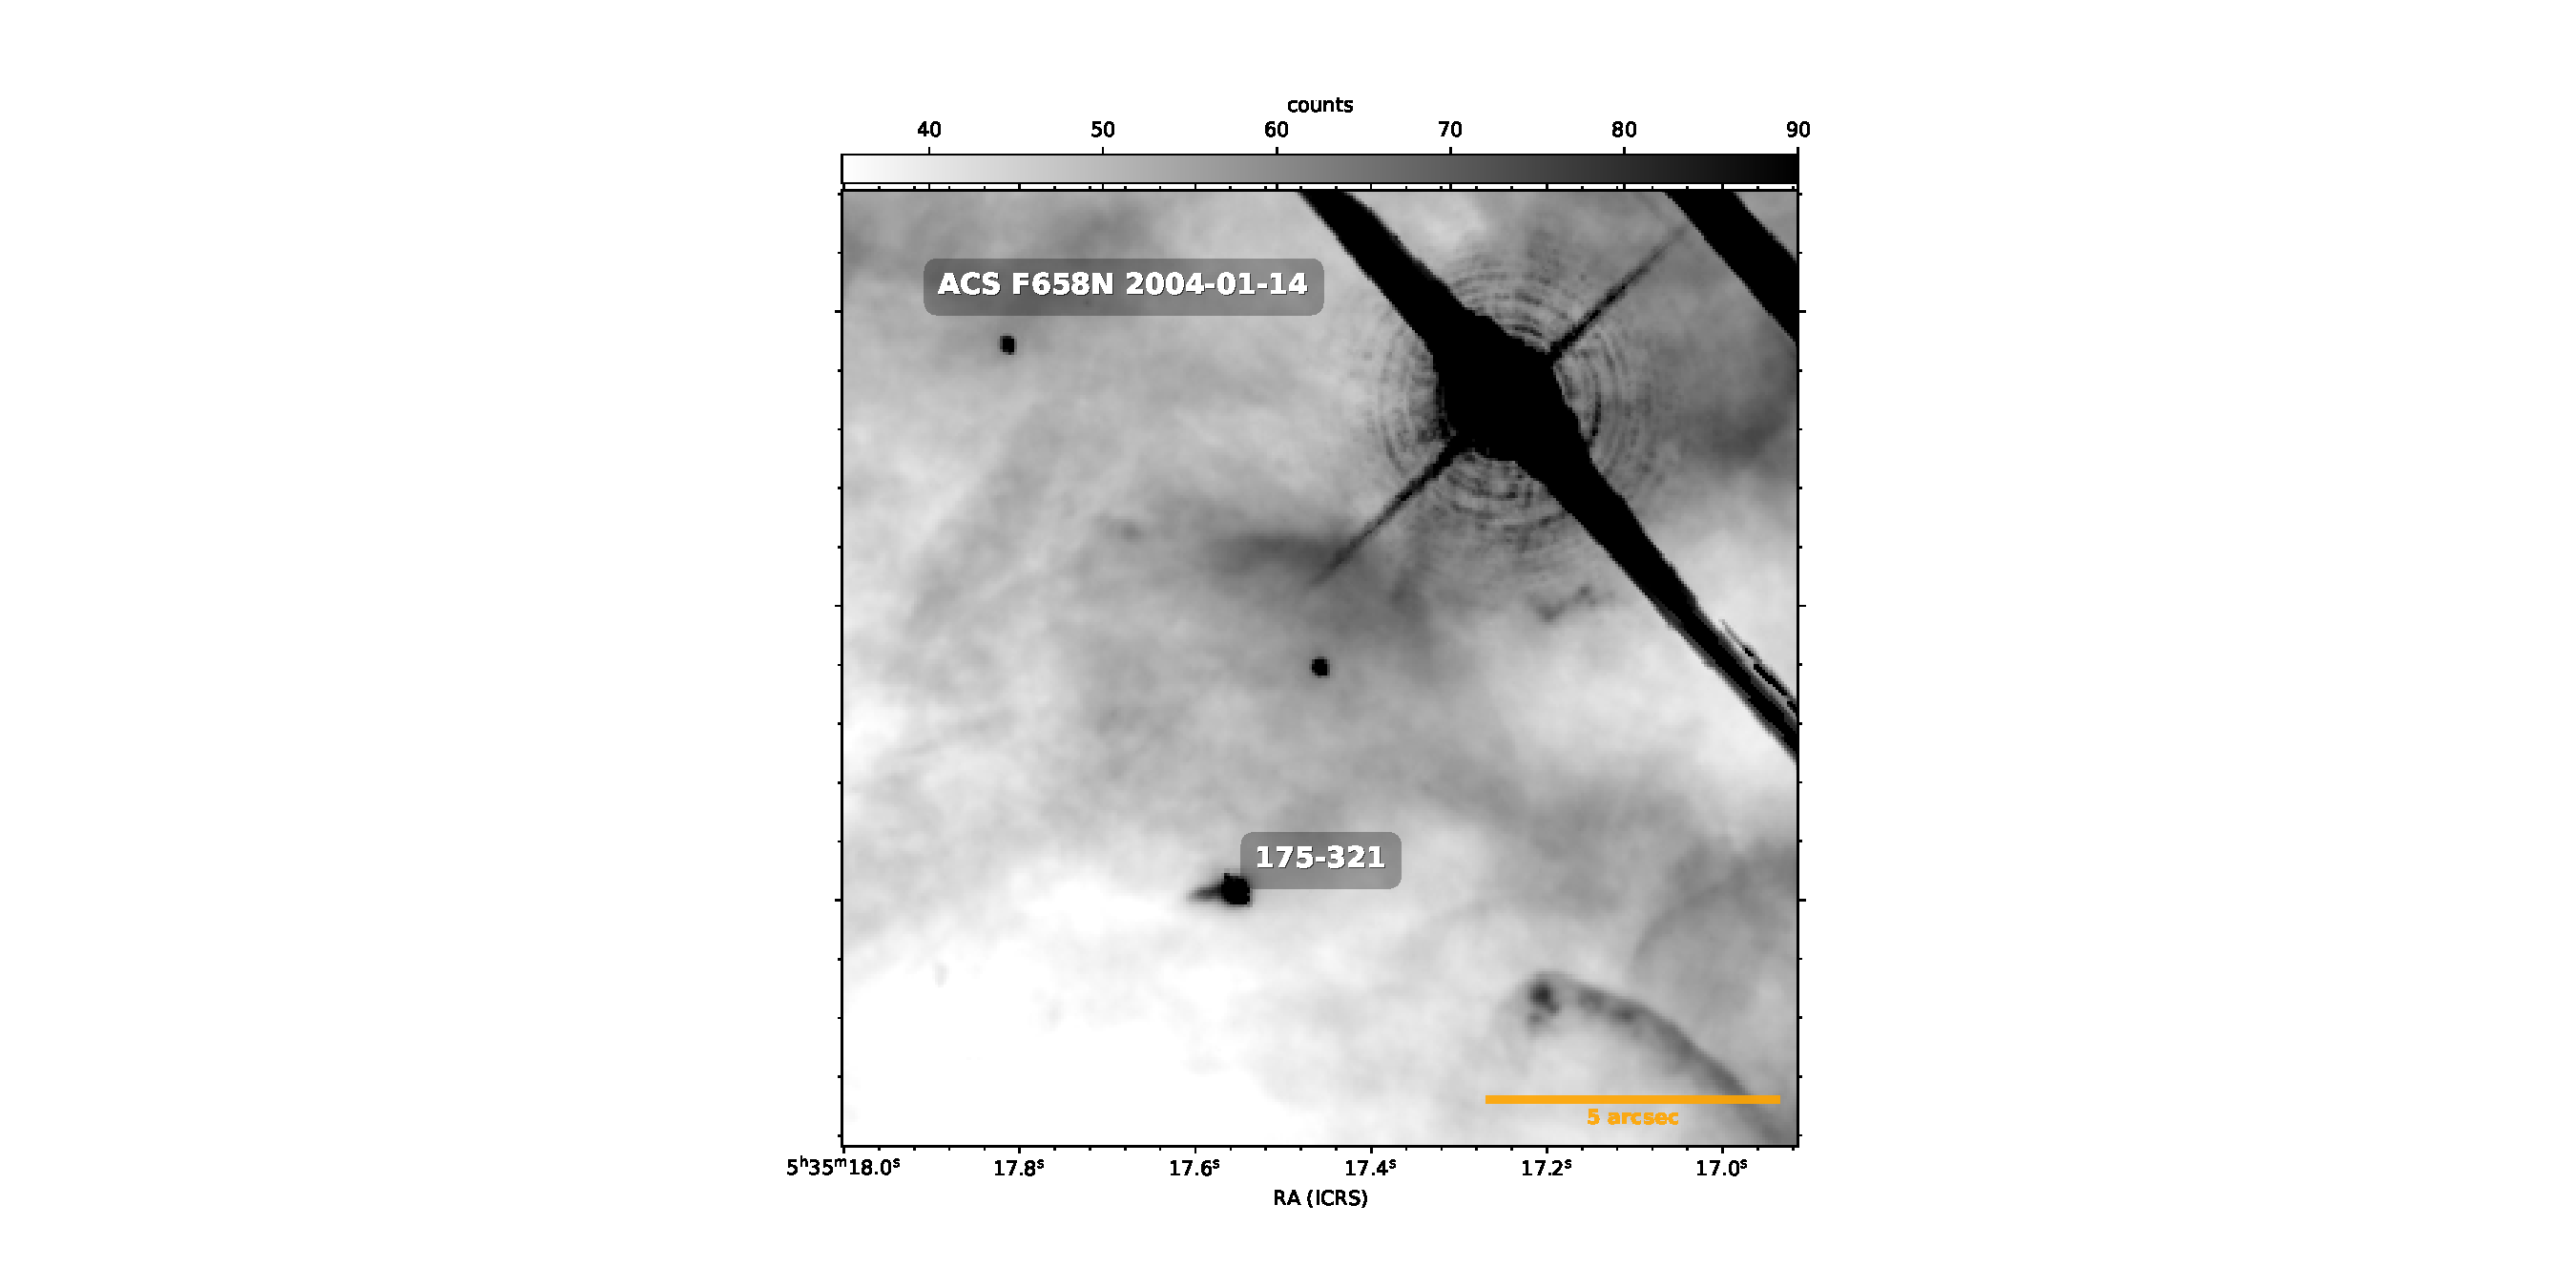
\includegraphics[width=0.165\linewidth, trim=350 10 350 40, clip]{175-321-Bally_01-images-simple} & 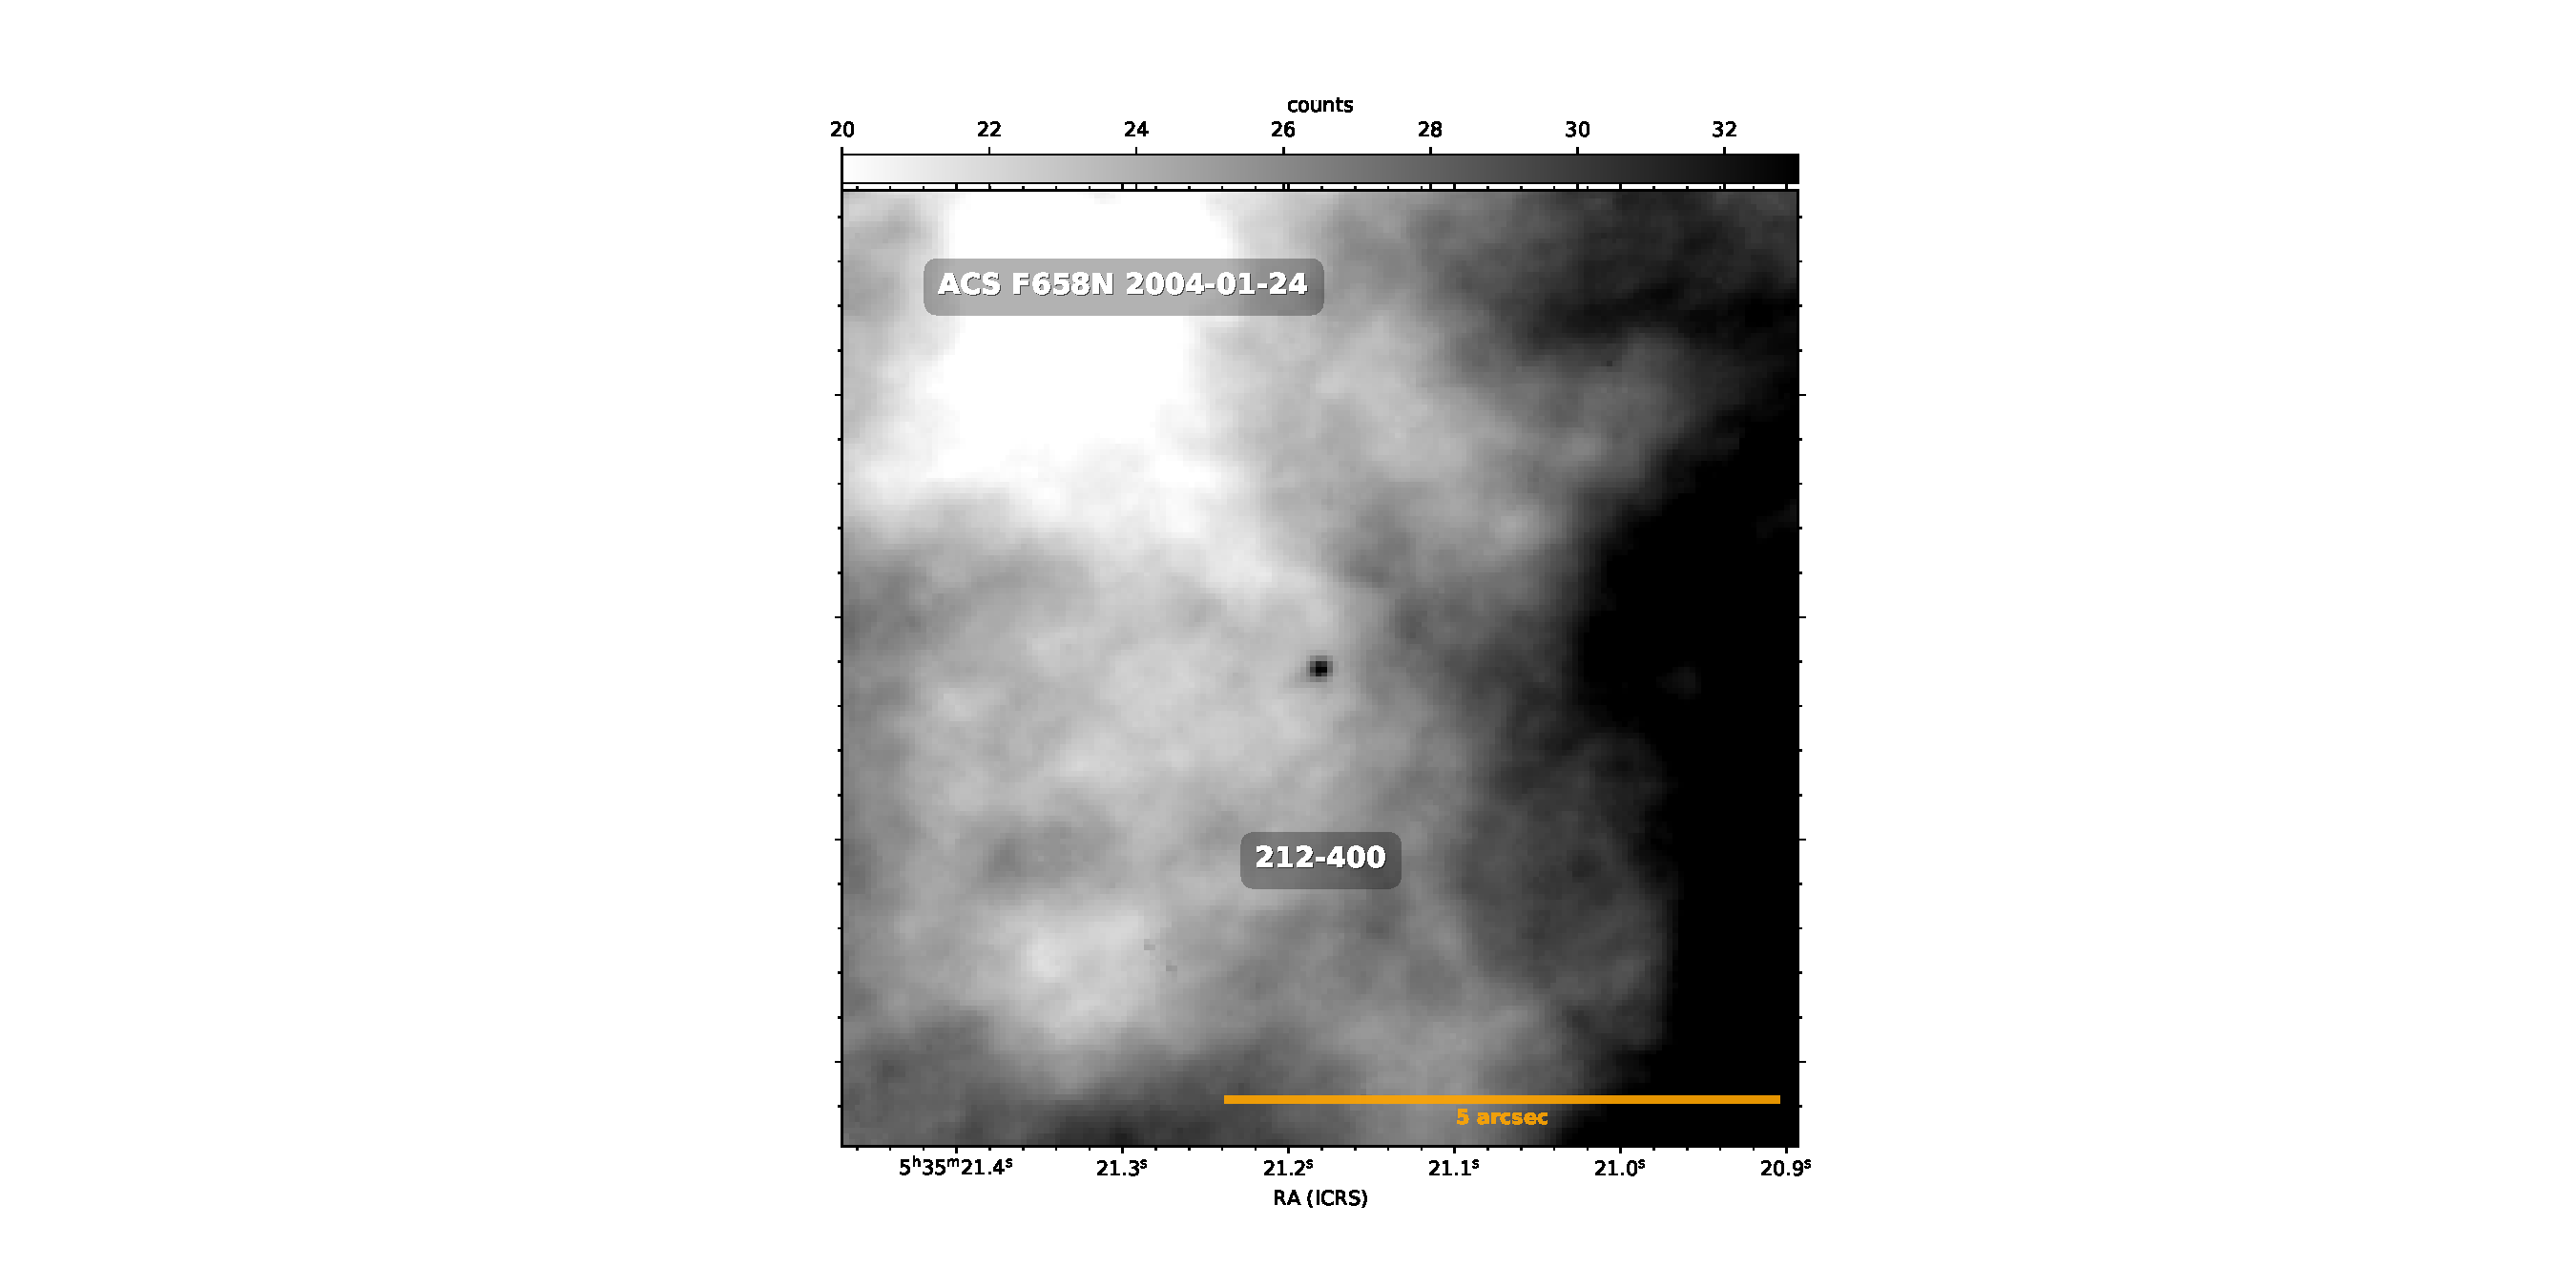
\includegraphics[width=0.165\linewidth, trim=350 10 350 40, clip]{212-400-Bally_06-images-simple} \\
    \raiselabel{(\textit{a})} & \raiselabel{(\textit{b})} \\
& &\multicolumn{2}{c}{\it  North group} \\
    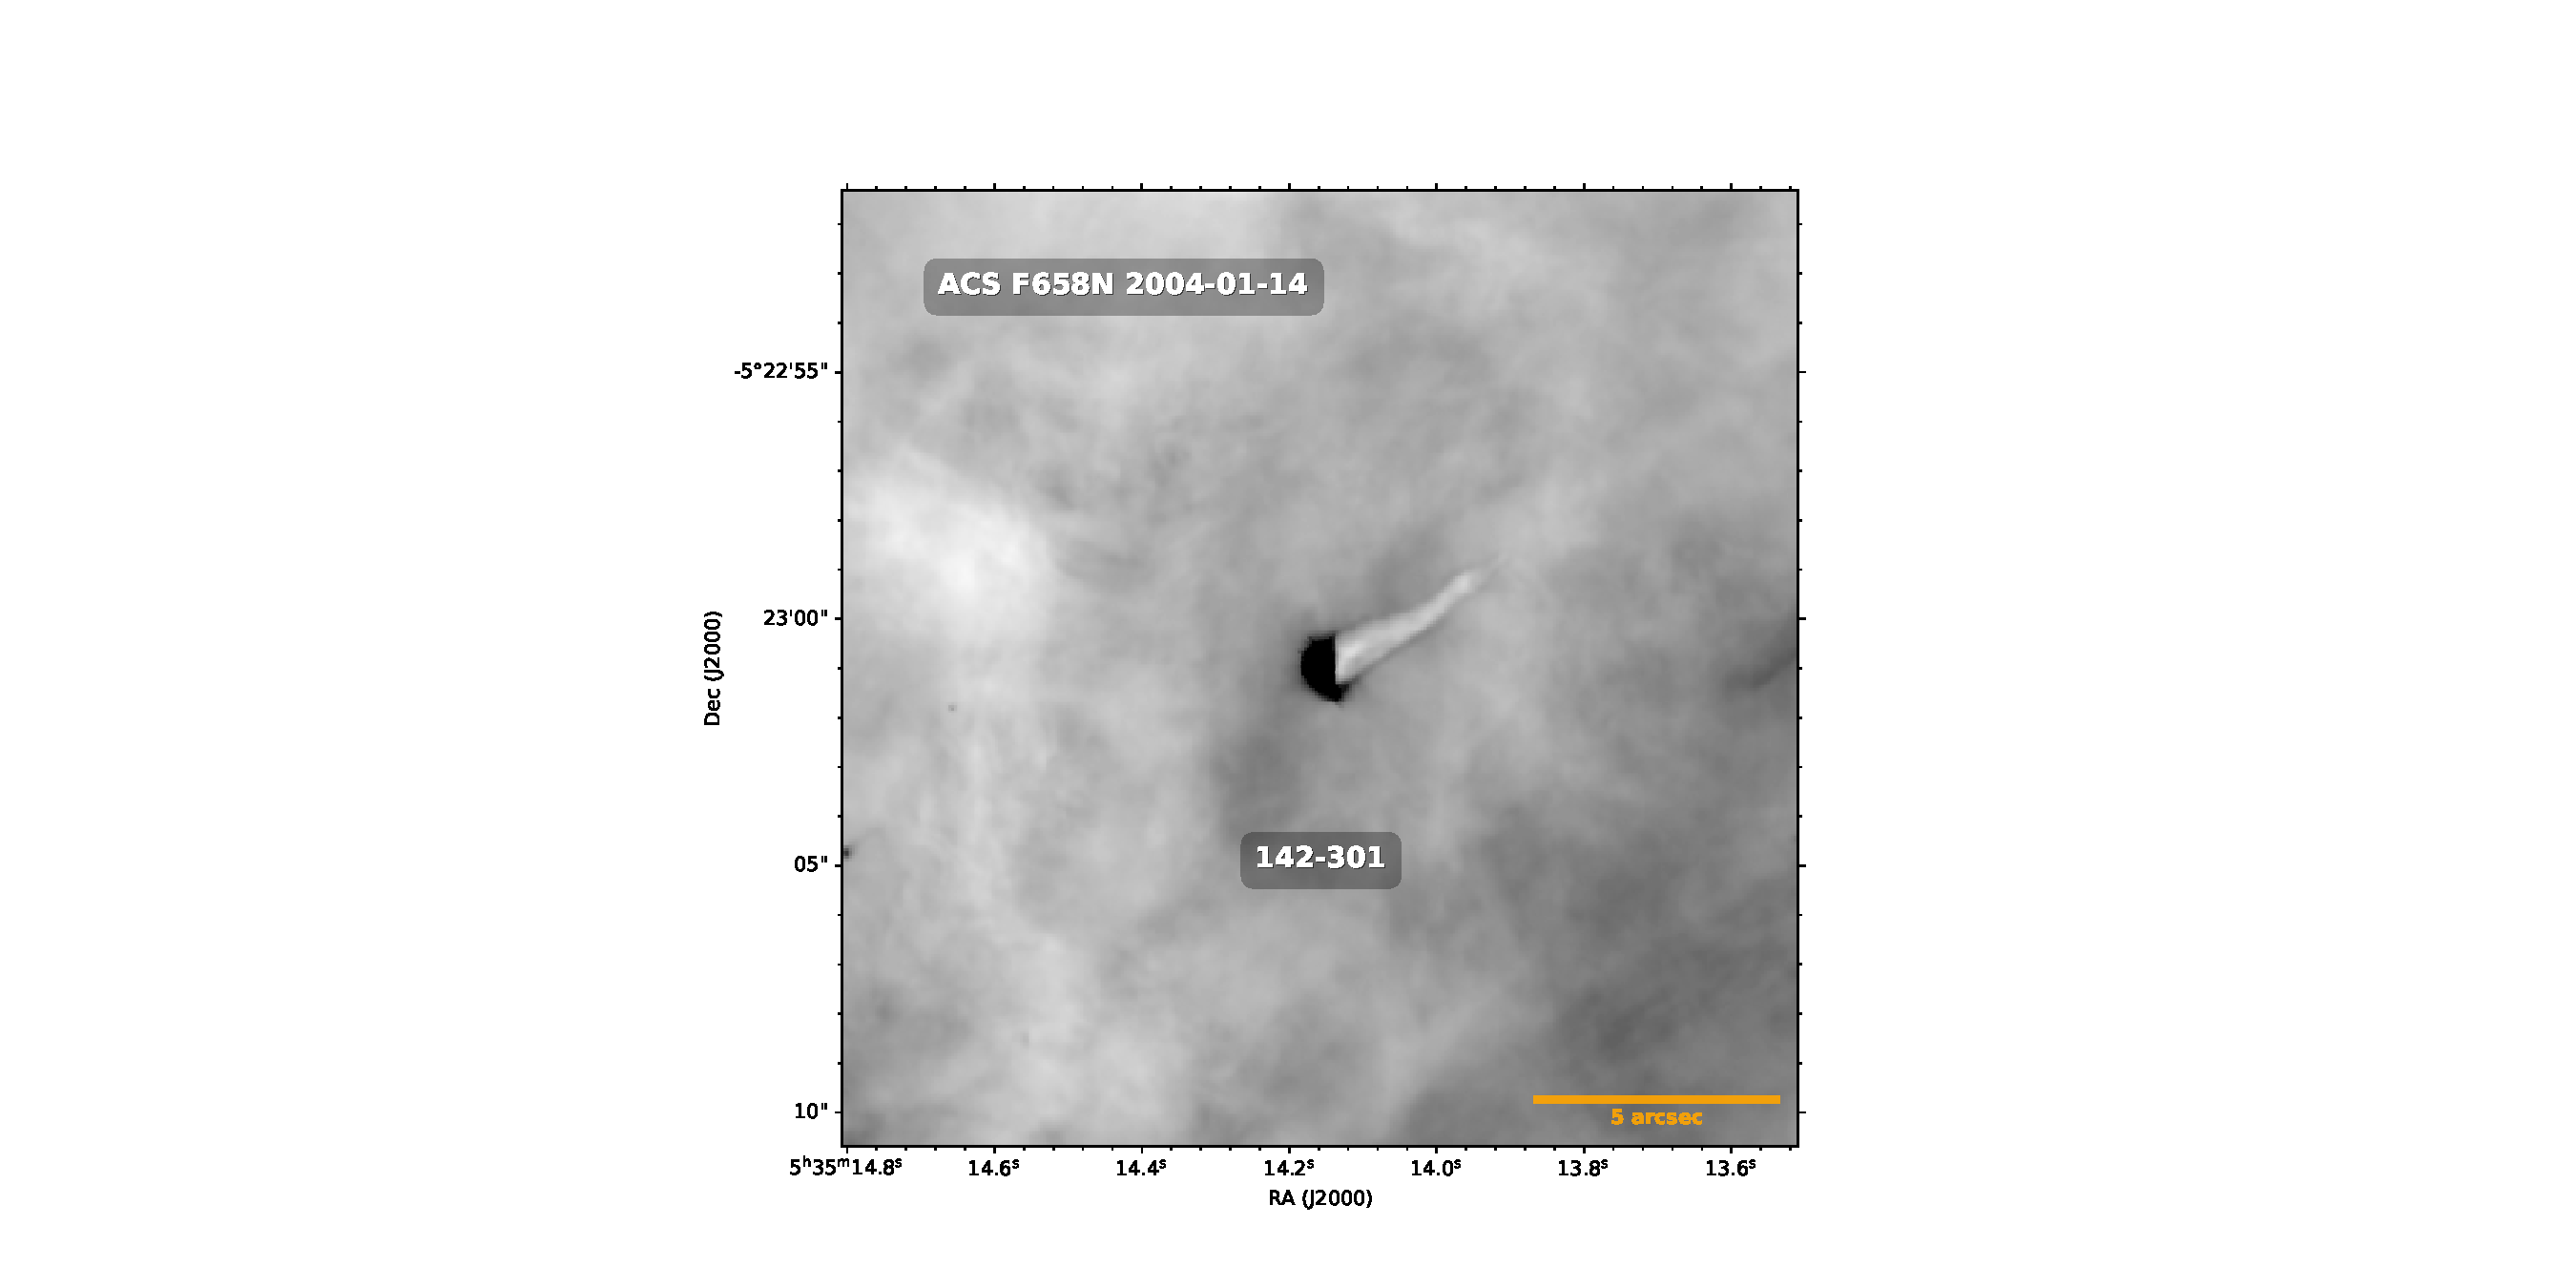
\includegraphics[width=0.165\linewidth, trim=350 10 350 40, clip]{142-301-Bally_01-images-simple} & 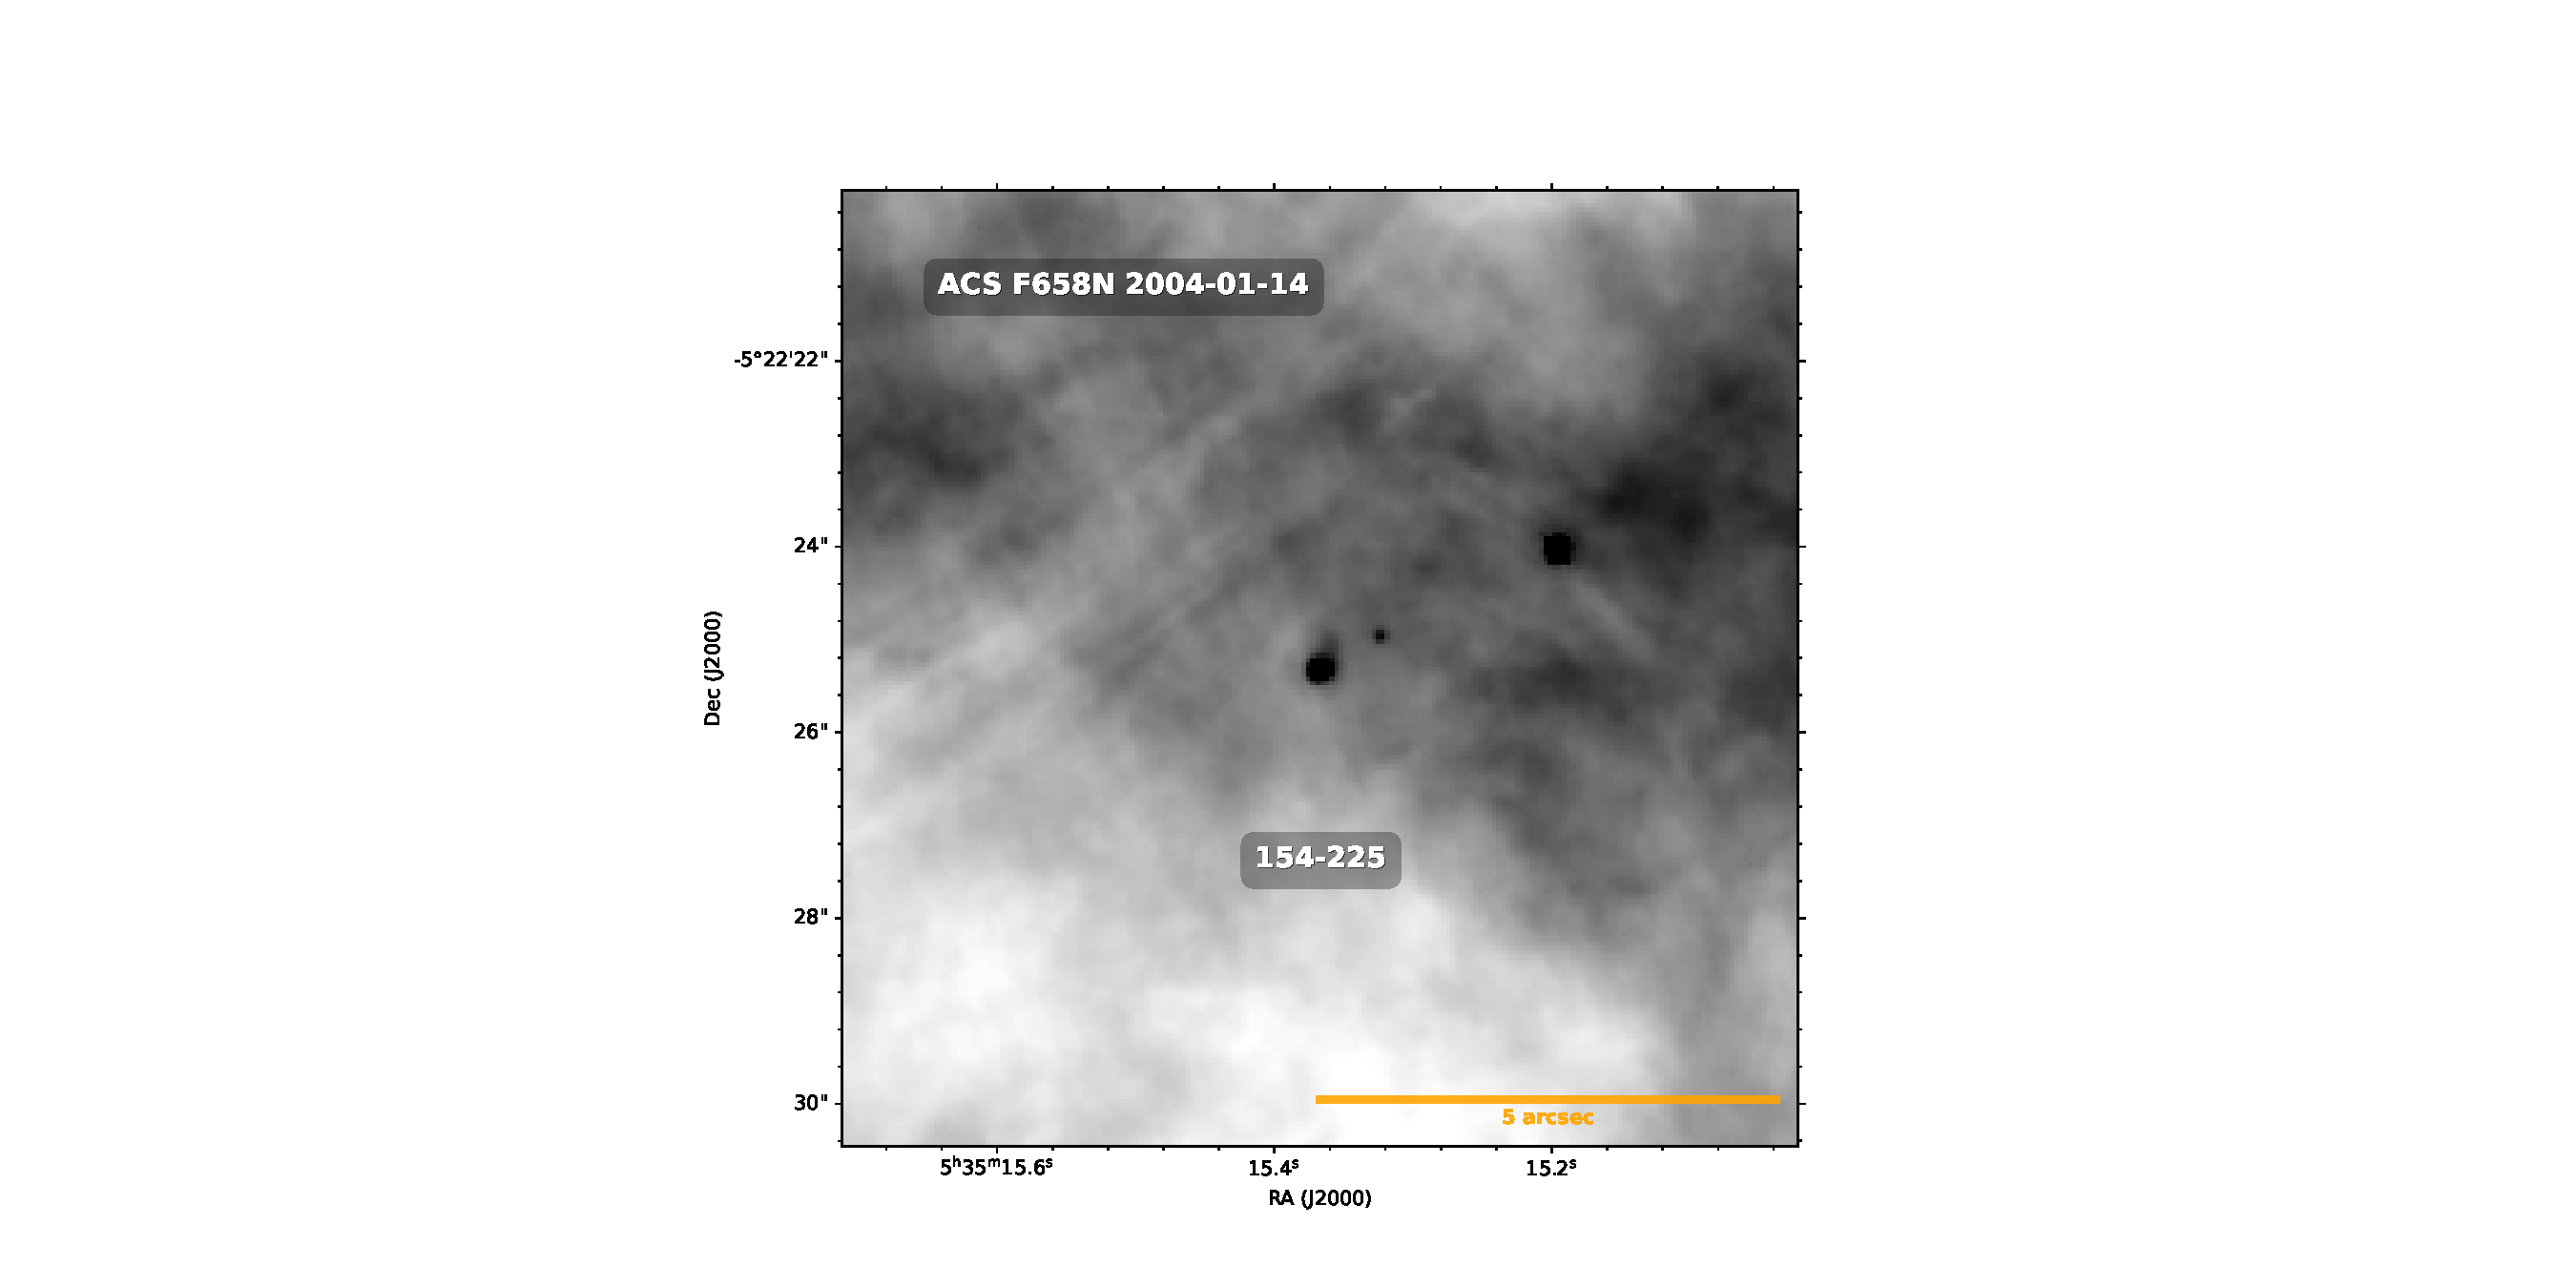
\includegraphics[width=0.165\linewidth, trim=350 10 350 40, clip]{154-225-Bally_01-images-simple} & 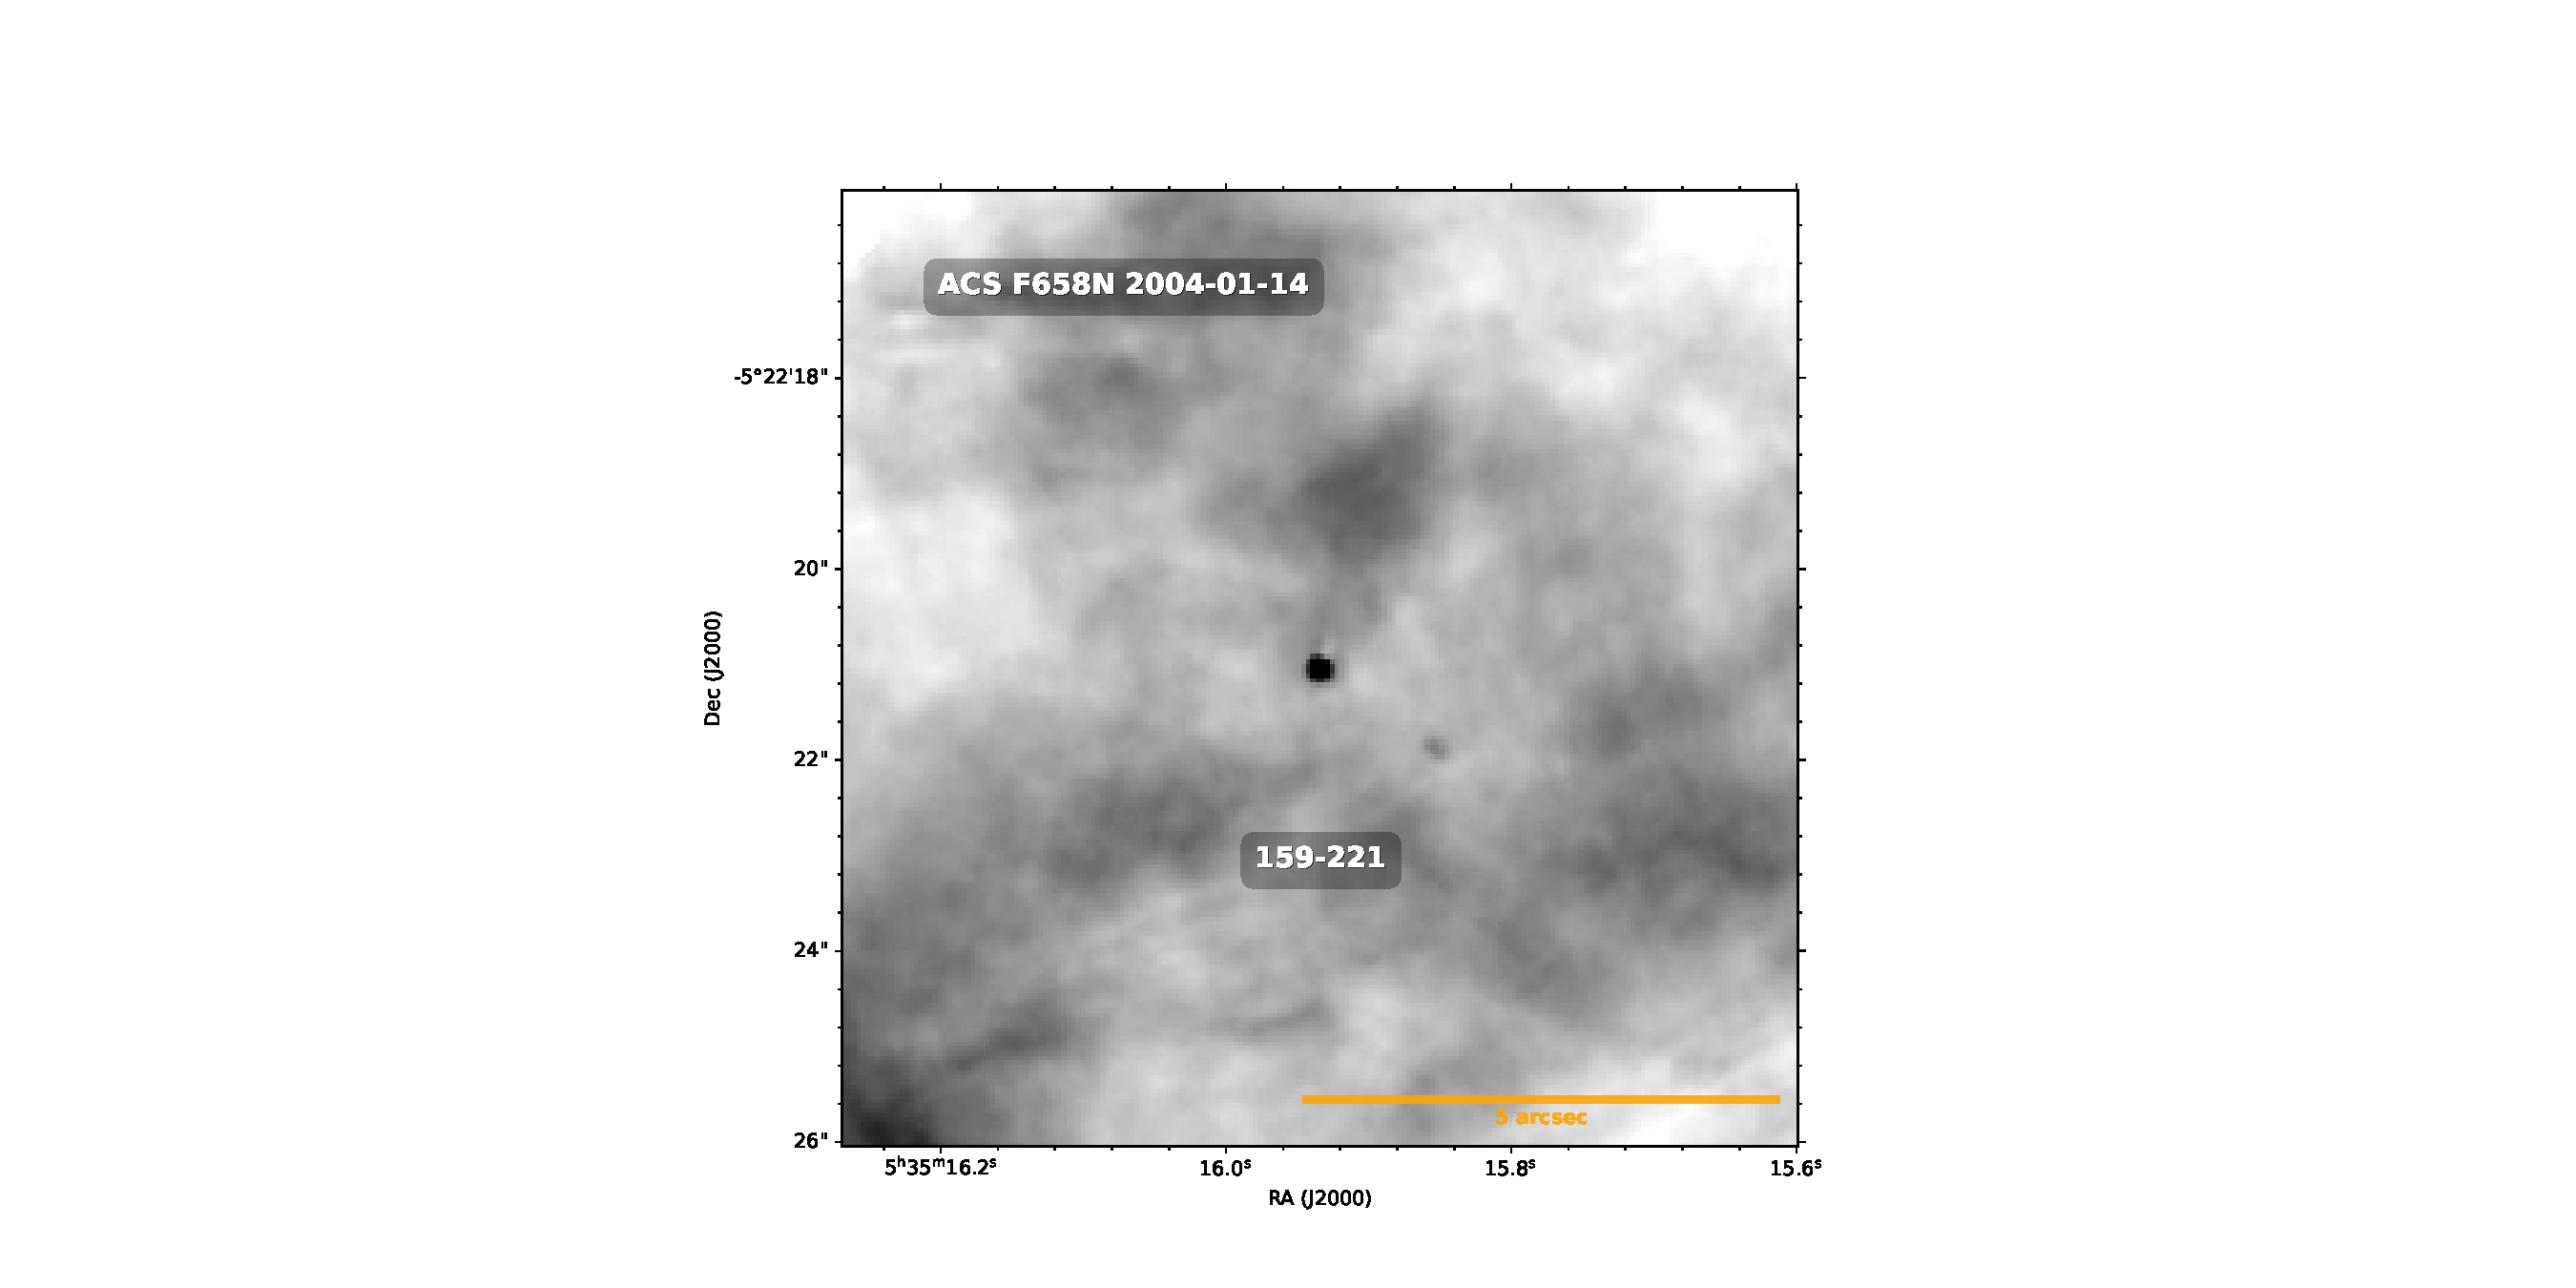
\includegraphics[width=0.165\linewidth, trim=350 10 350 40, clip]{159-221-Bally_01-images-simple} & 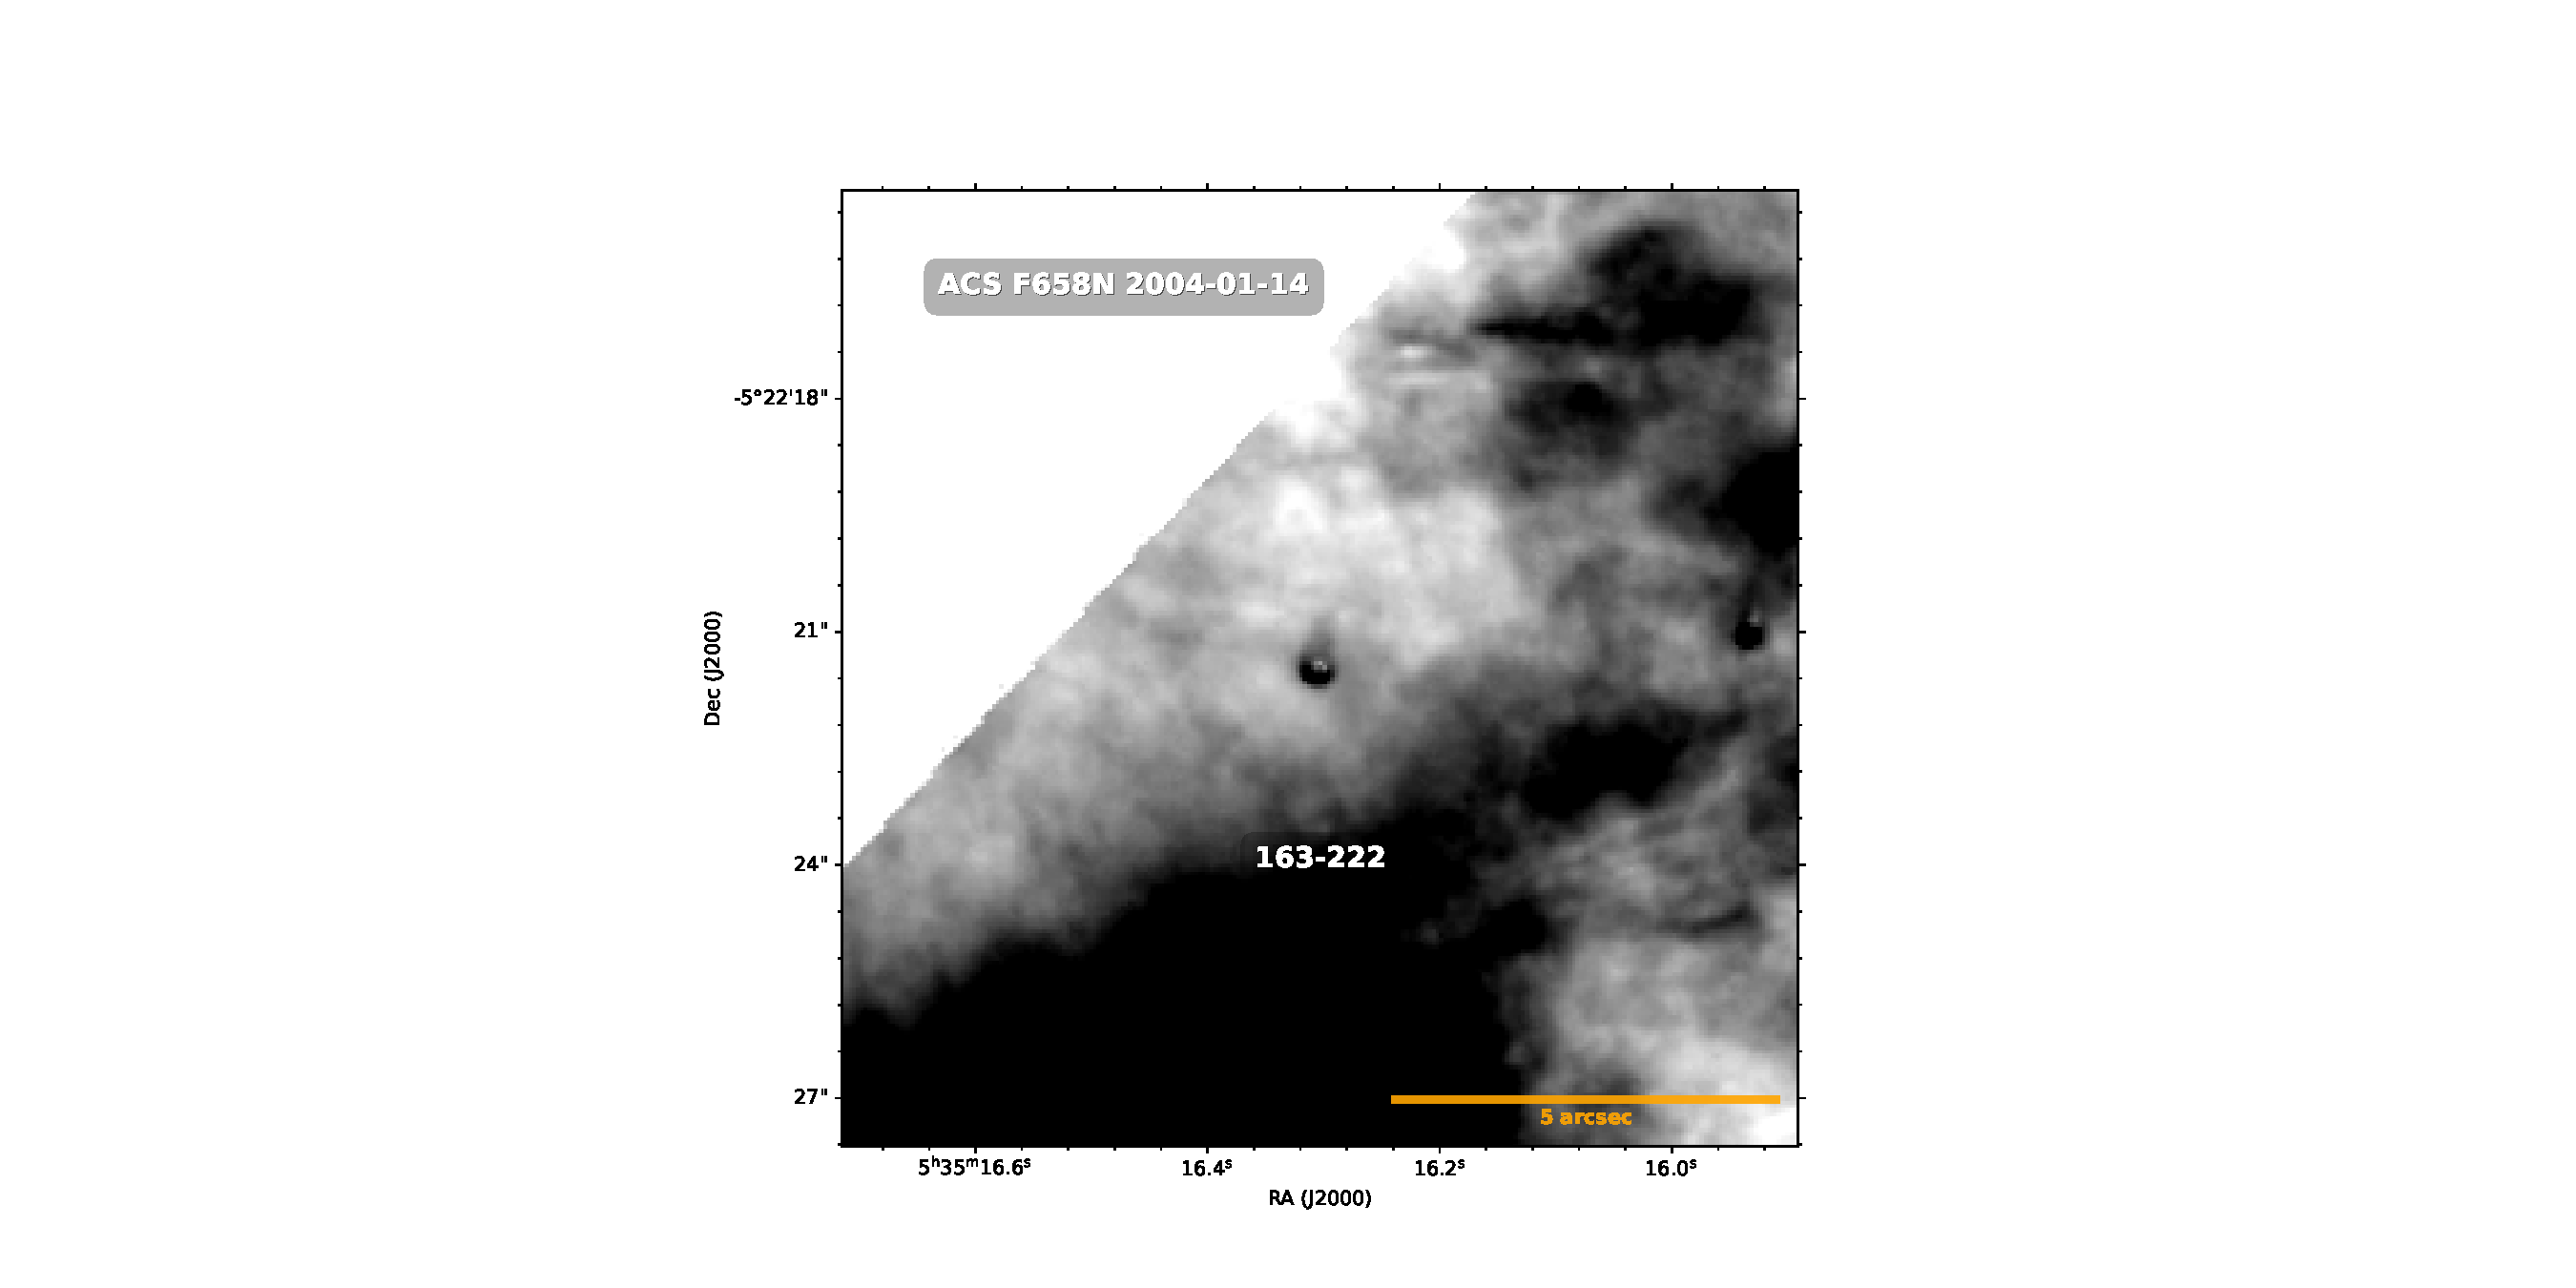
\includegraphics[width=0.165\linewidth, trim=350 10 350 40, clip]{163-222-Bally_01-images-simple} & 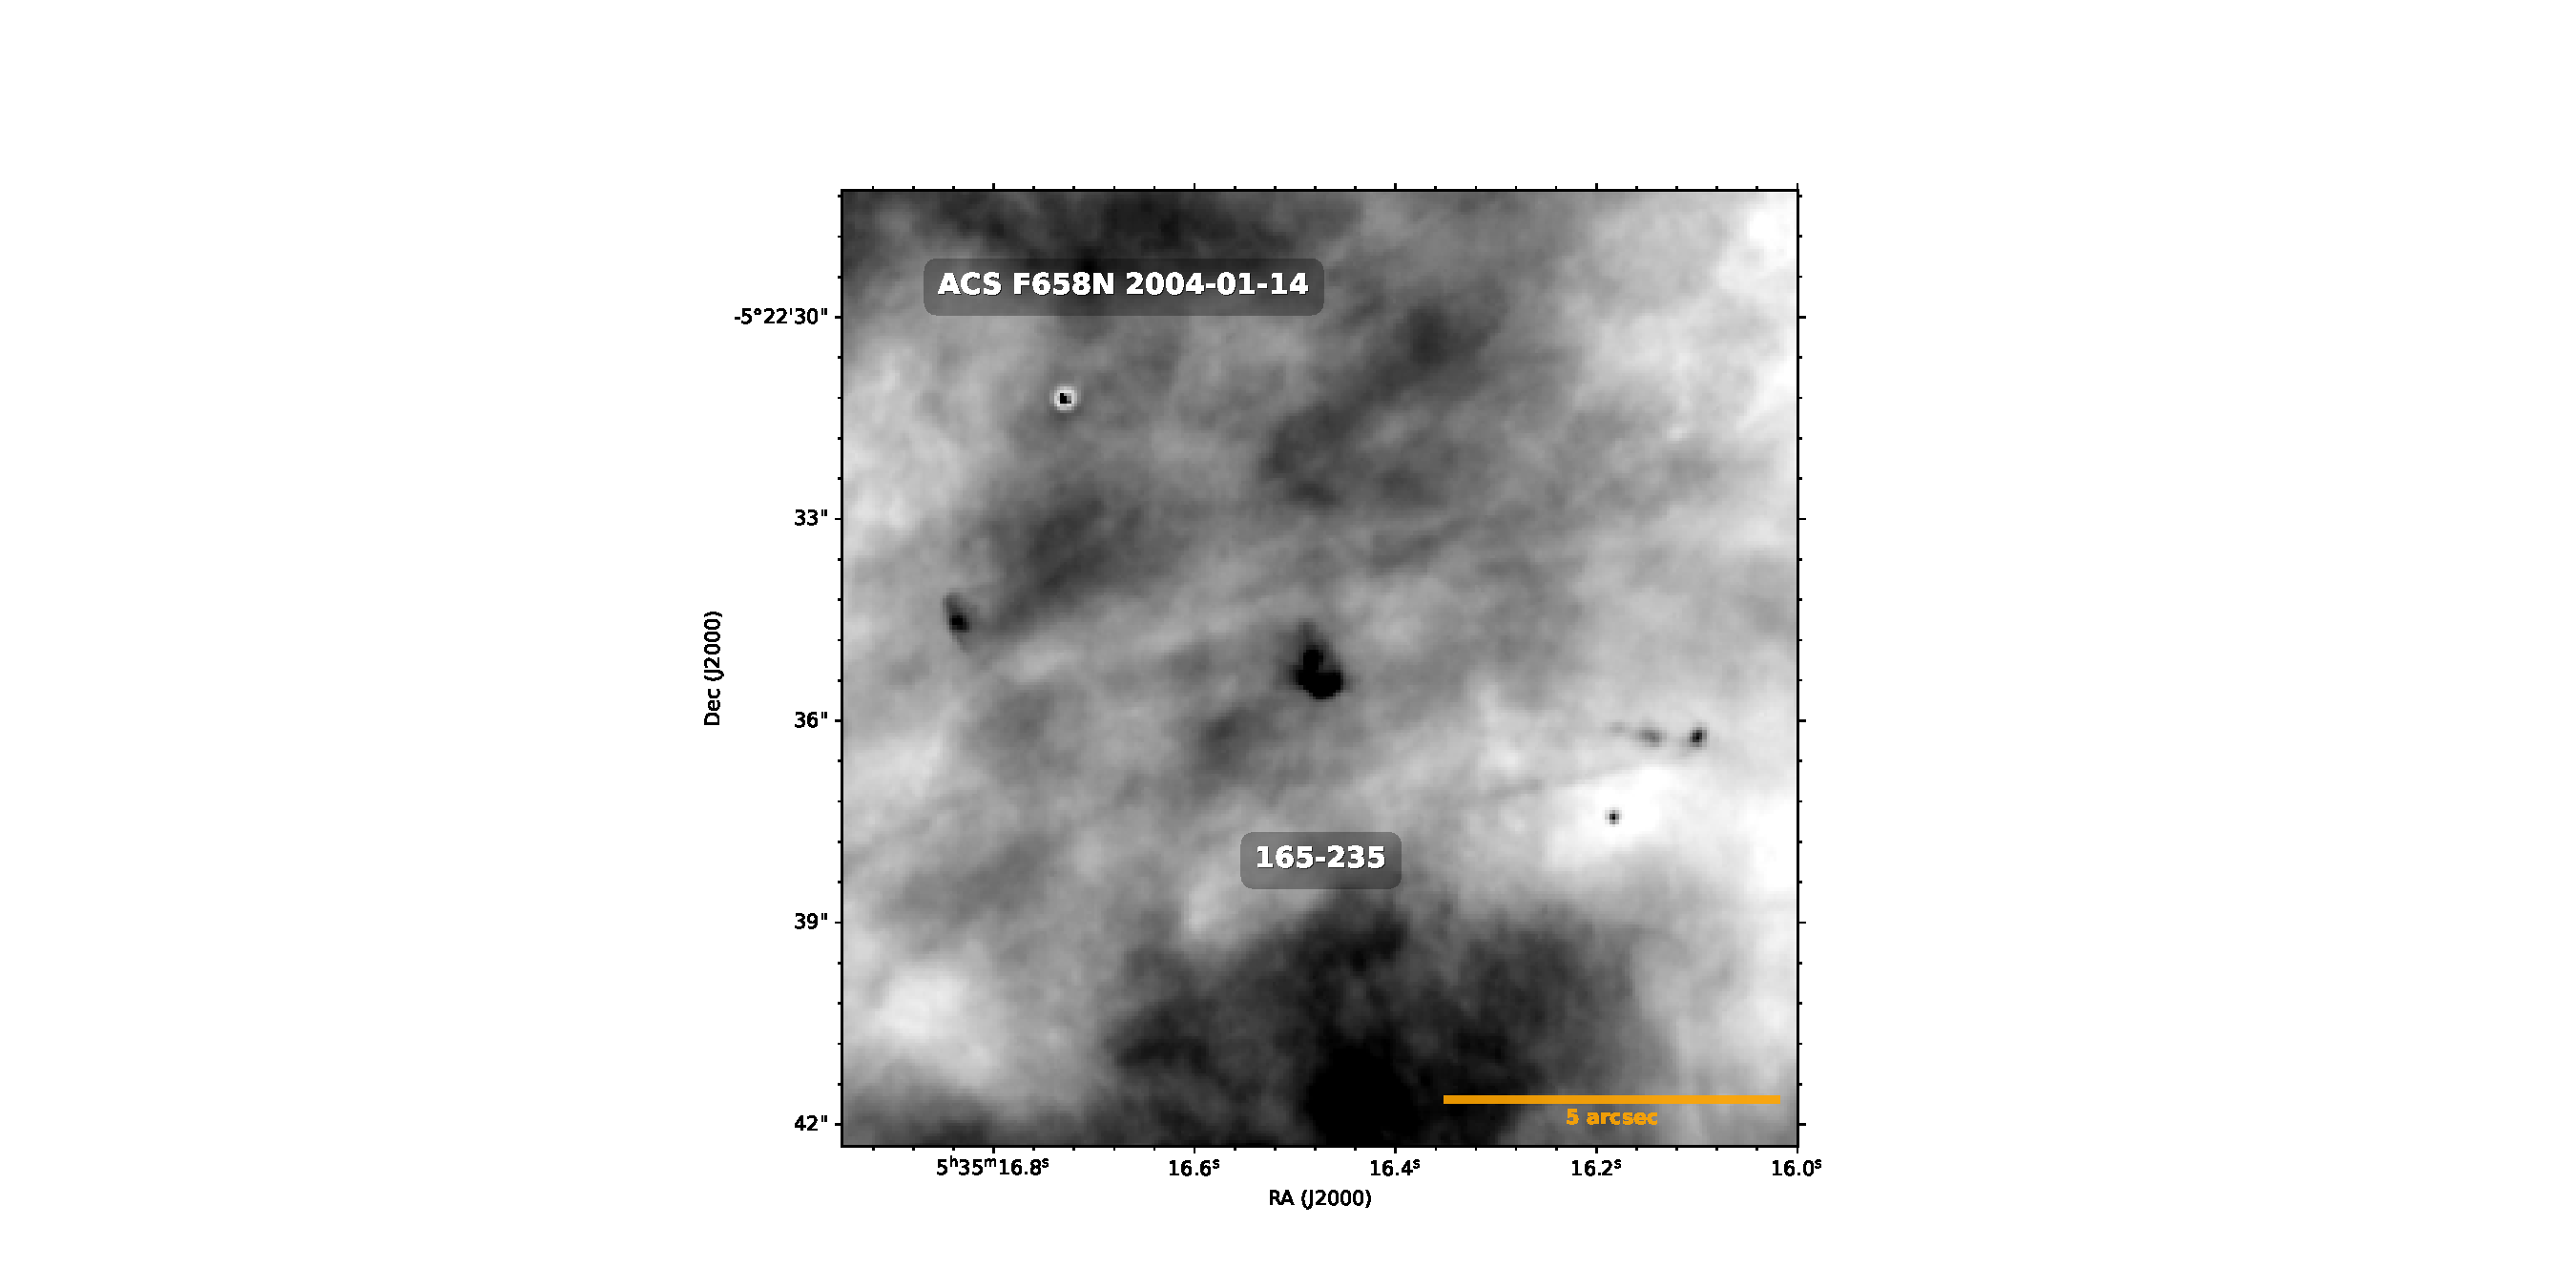
\includegraphics[width=0.165\linewidth, trim=350 10 350 40, clip]{165-235-Bally_01-images-simple} \\
    \raiselabel{(\textit{c})} & \raiselabel{(\textit{d})} & \raiselabel{(\textit{e})} & \raiselabel{(\textit{f})} & \raiselabel{(\textit{g})} \\
    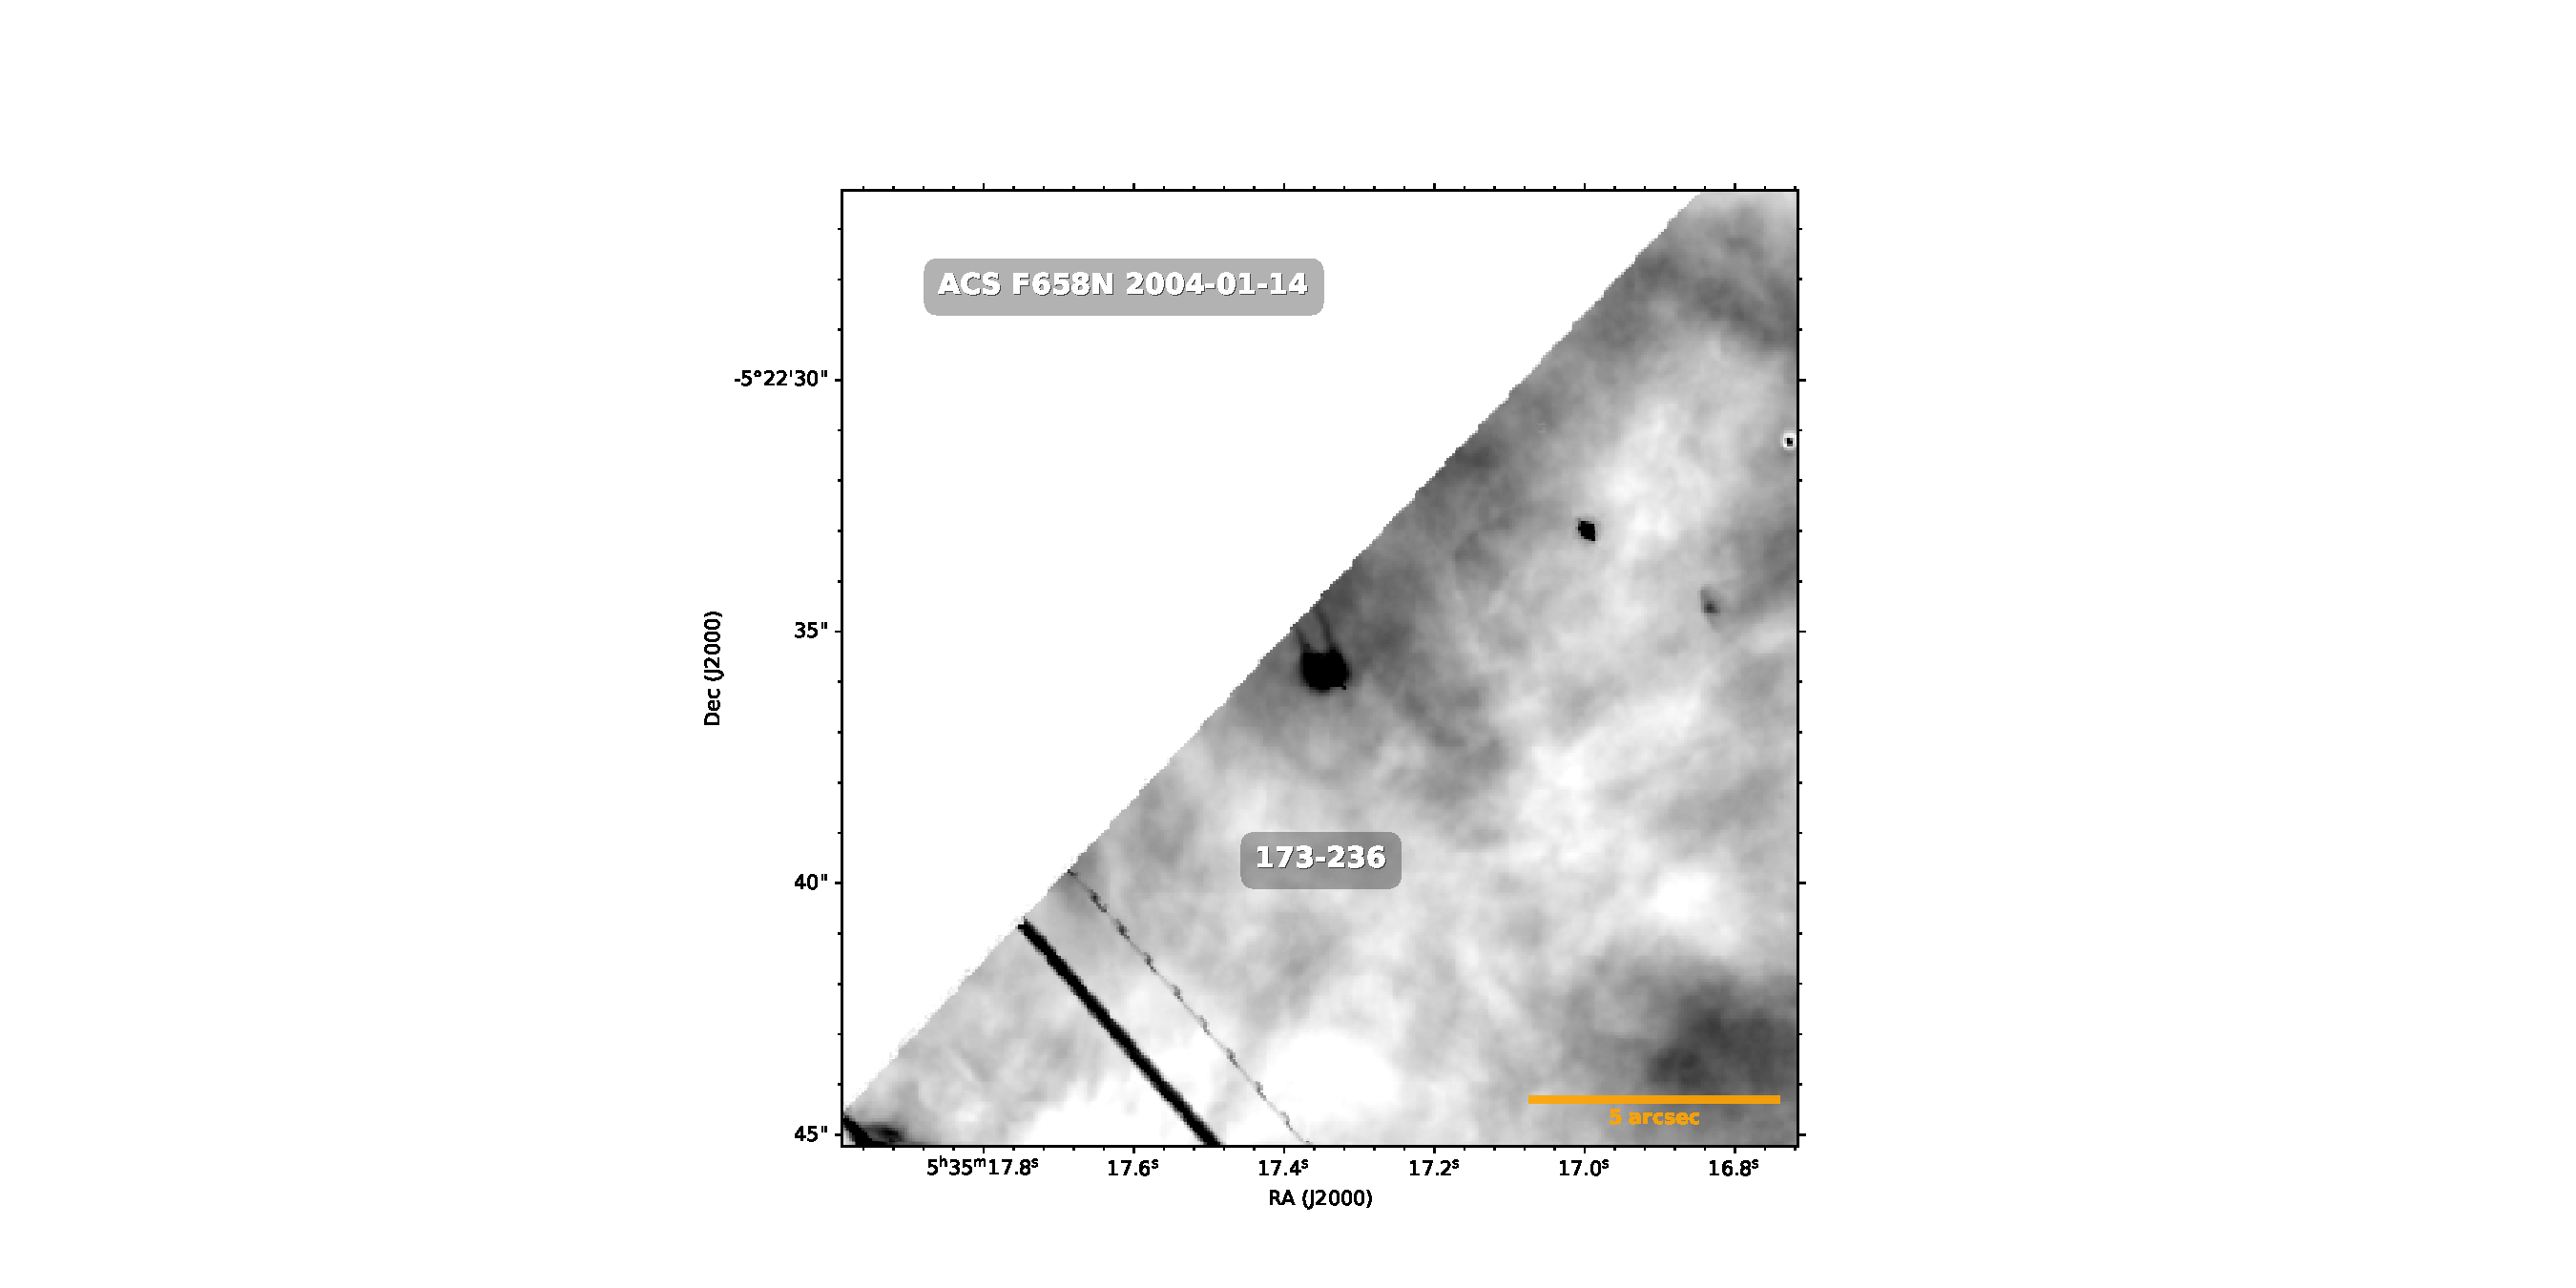
\includegraphics[width=0.165\linewidth, trim=350 10 350 40, clip]{173-236-Bally_01-images-simple} & 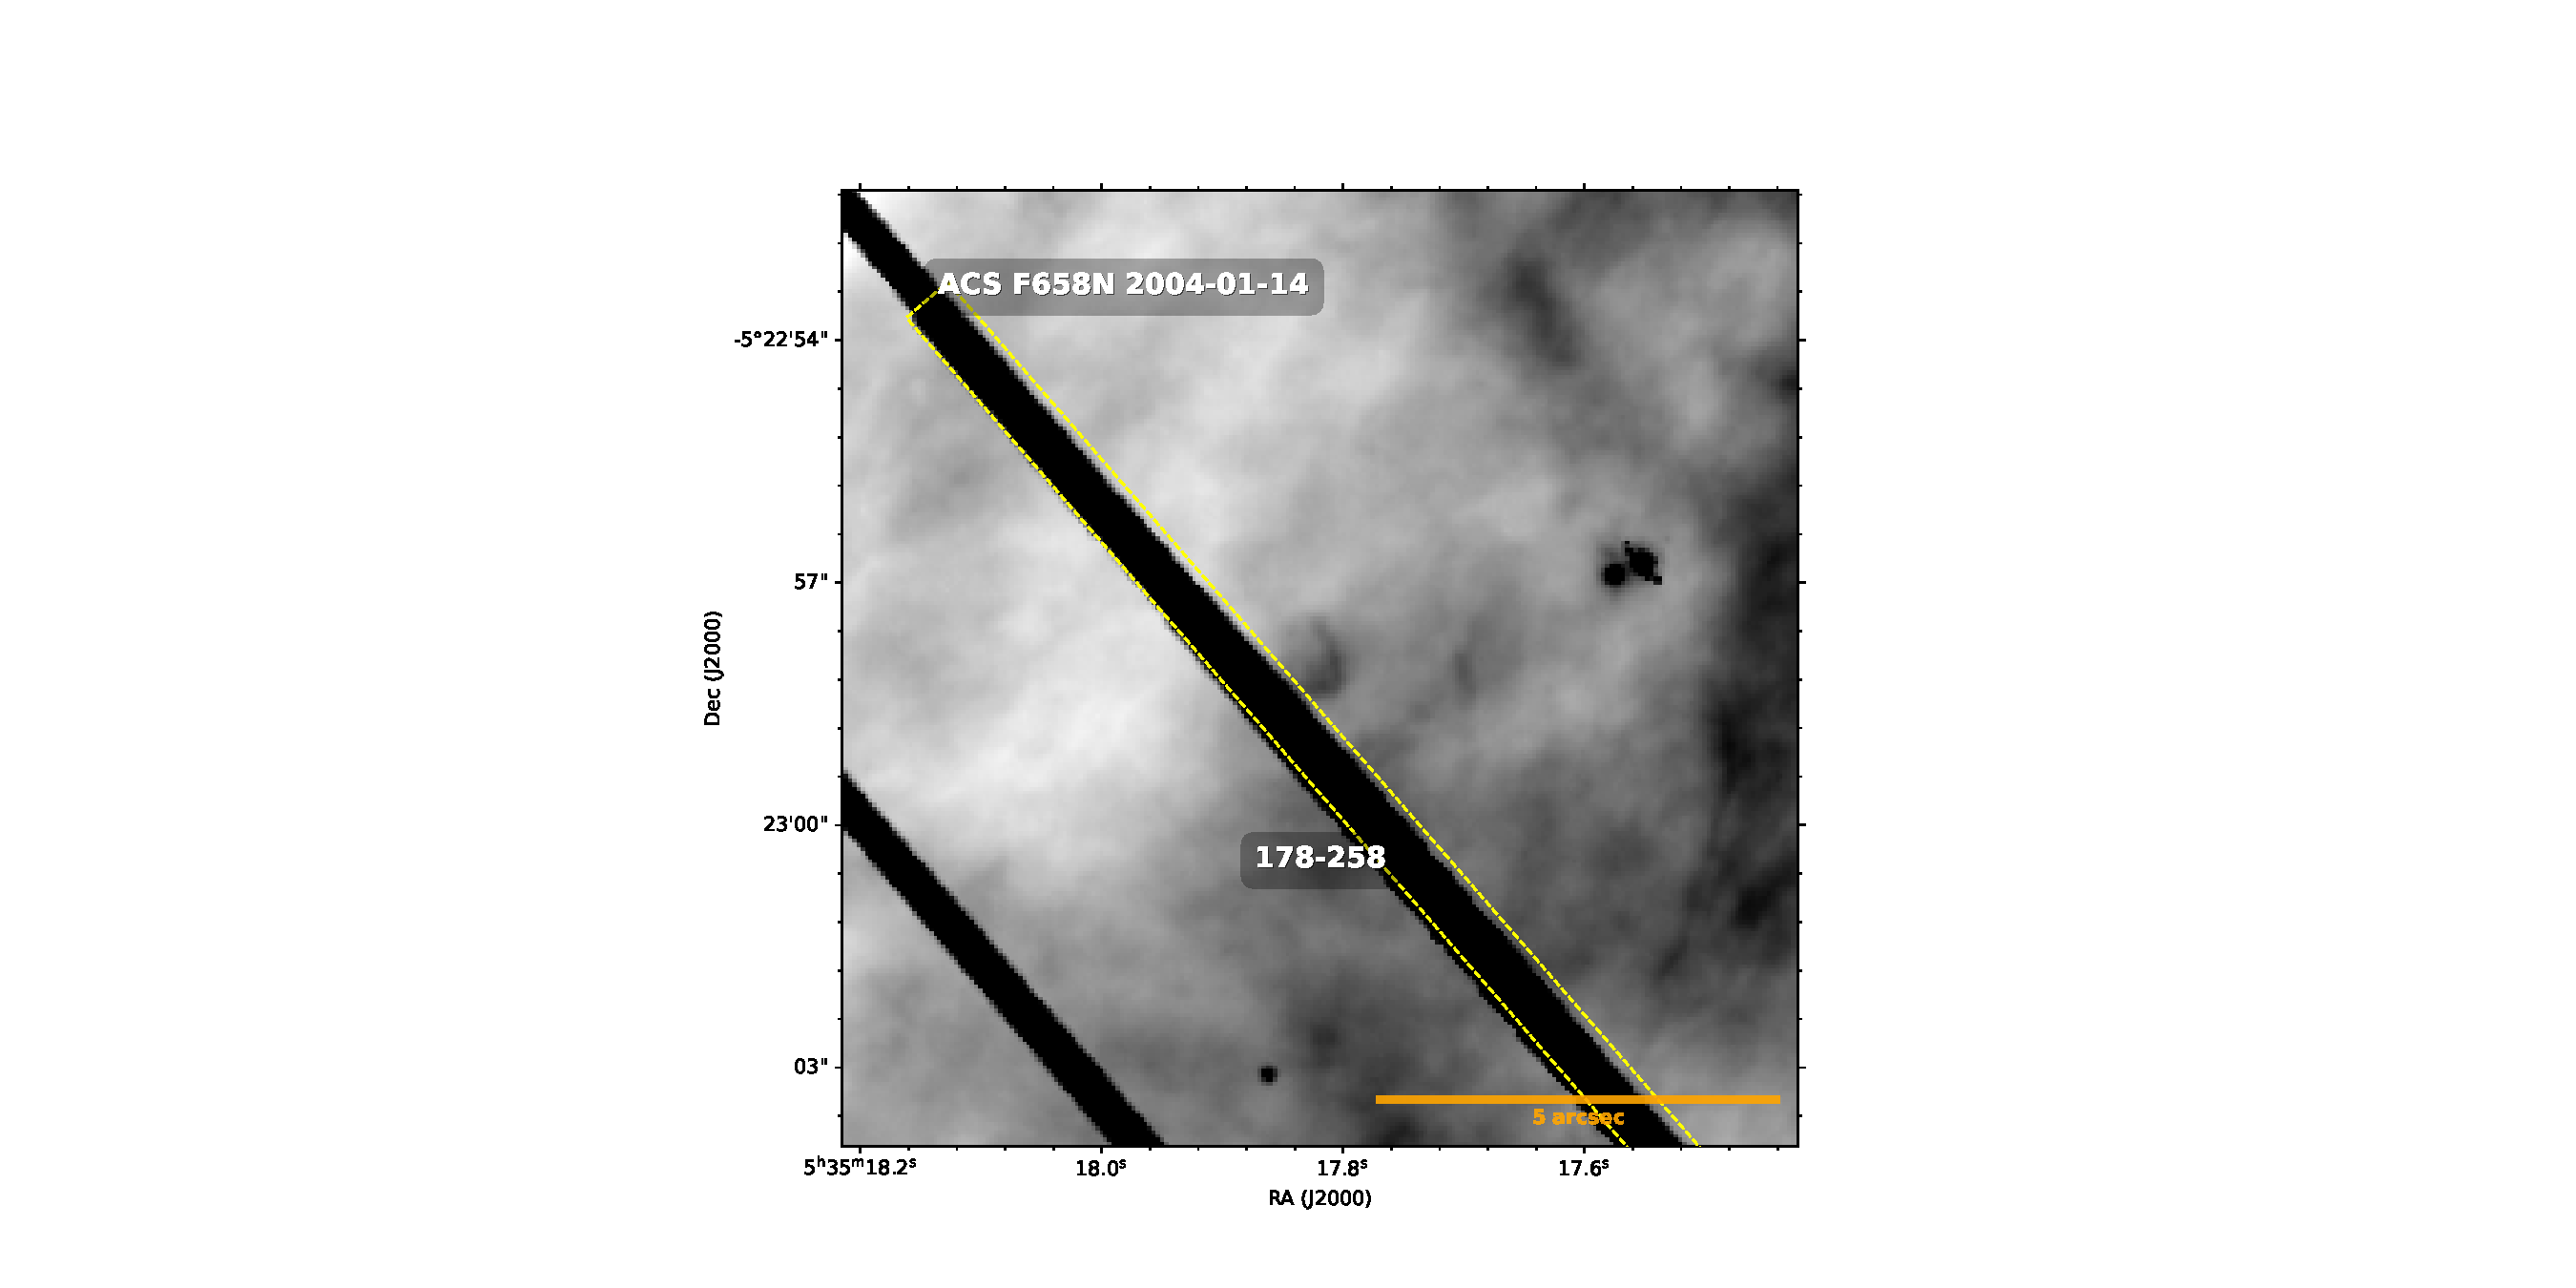
\includegraphics[width=0.165\linewidth, trim=350 10 350 40, clip]{178-258-Bally_01-images-simple} \\
    \raiselabel{(\textit{h})} & \raiselabel{(\textit{i})} \\
& &\multicolumn{2}{c}{\it  Northwest group} \\
    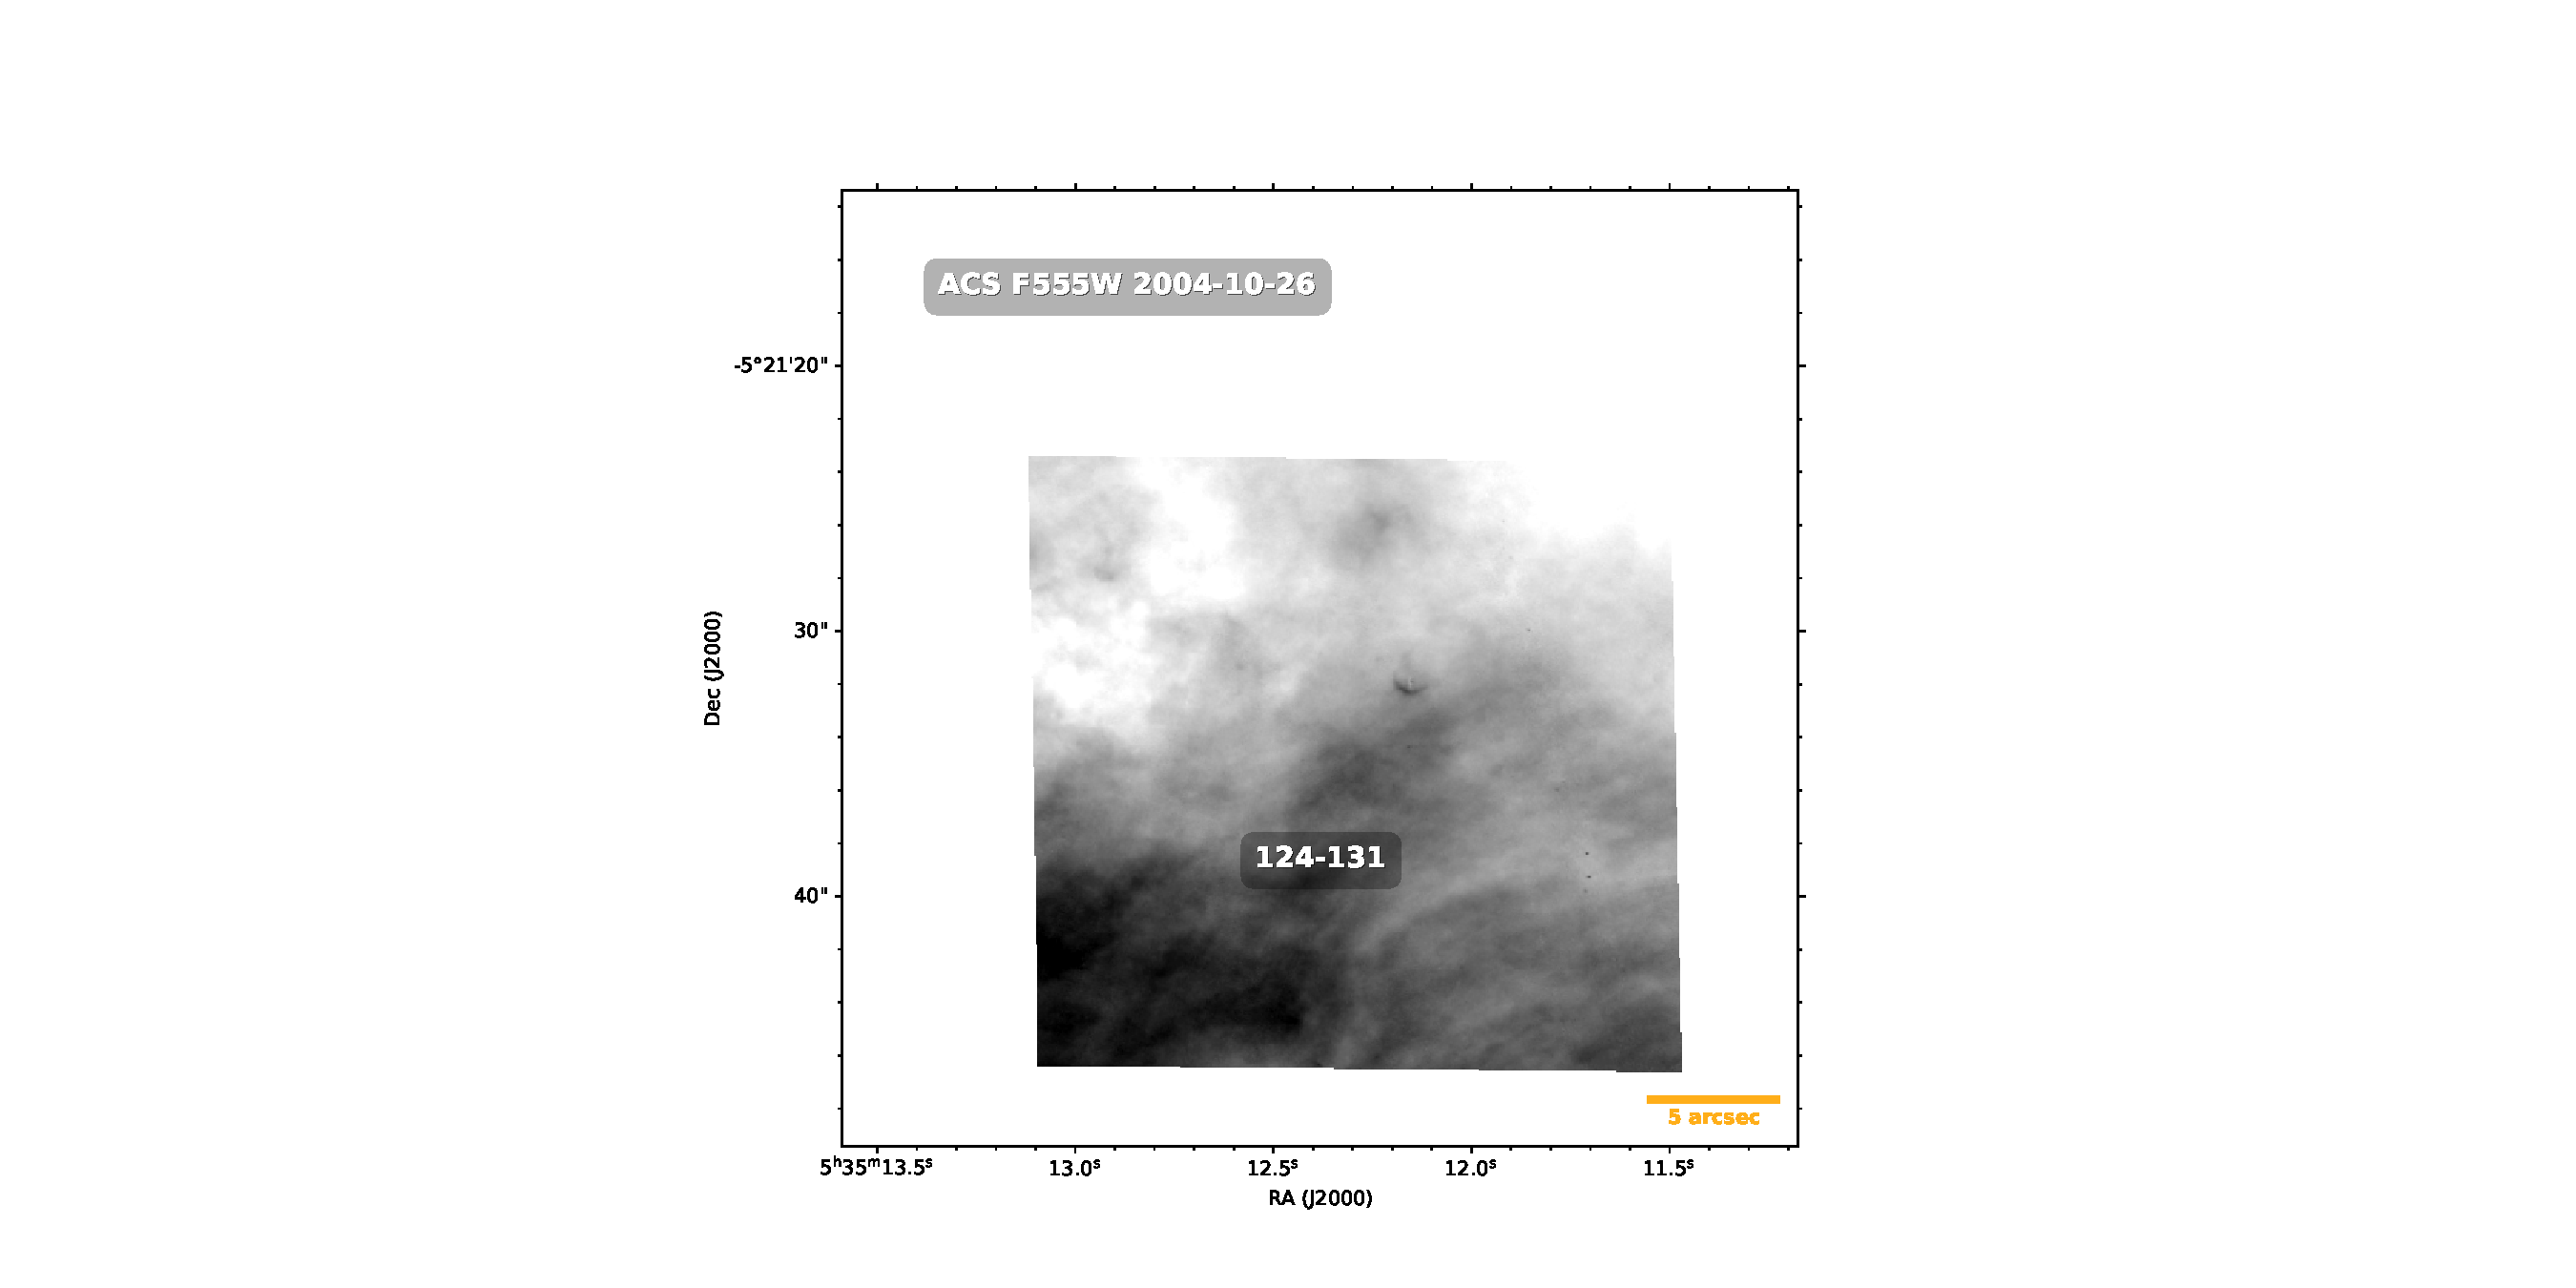
\includegraphics[width=0.165\linewidth, trim=350 10 350 40, clip]{124-131-Robberto_ACS_5l_f555w-images-simple} & 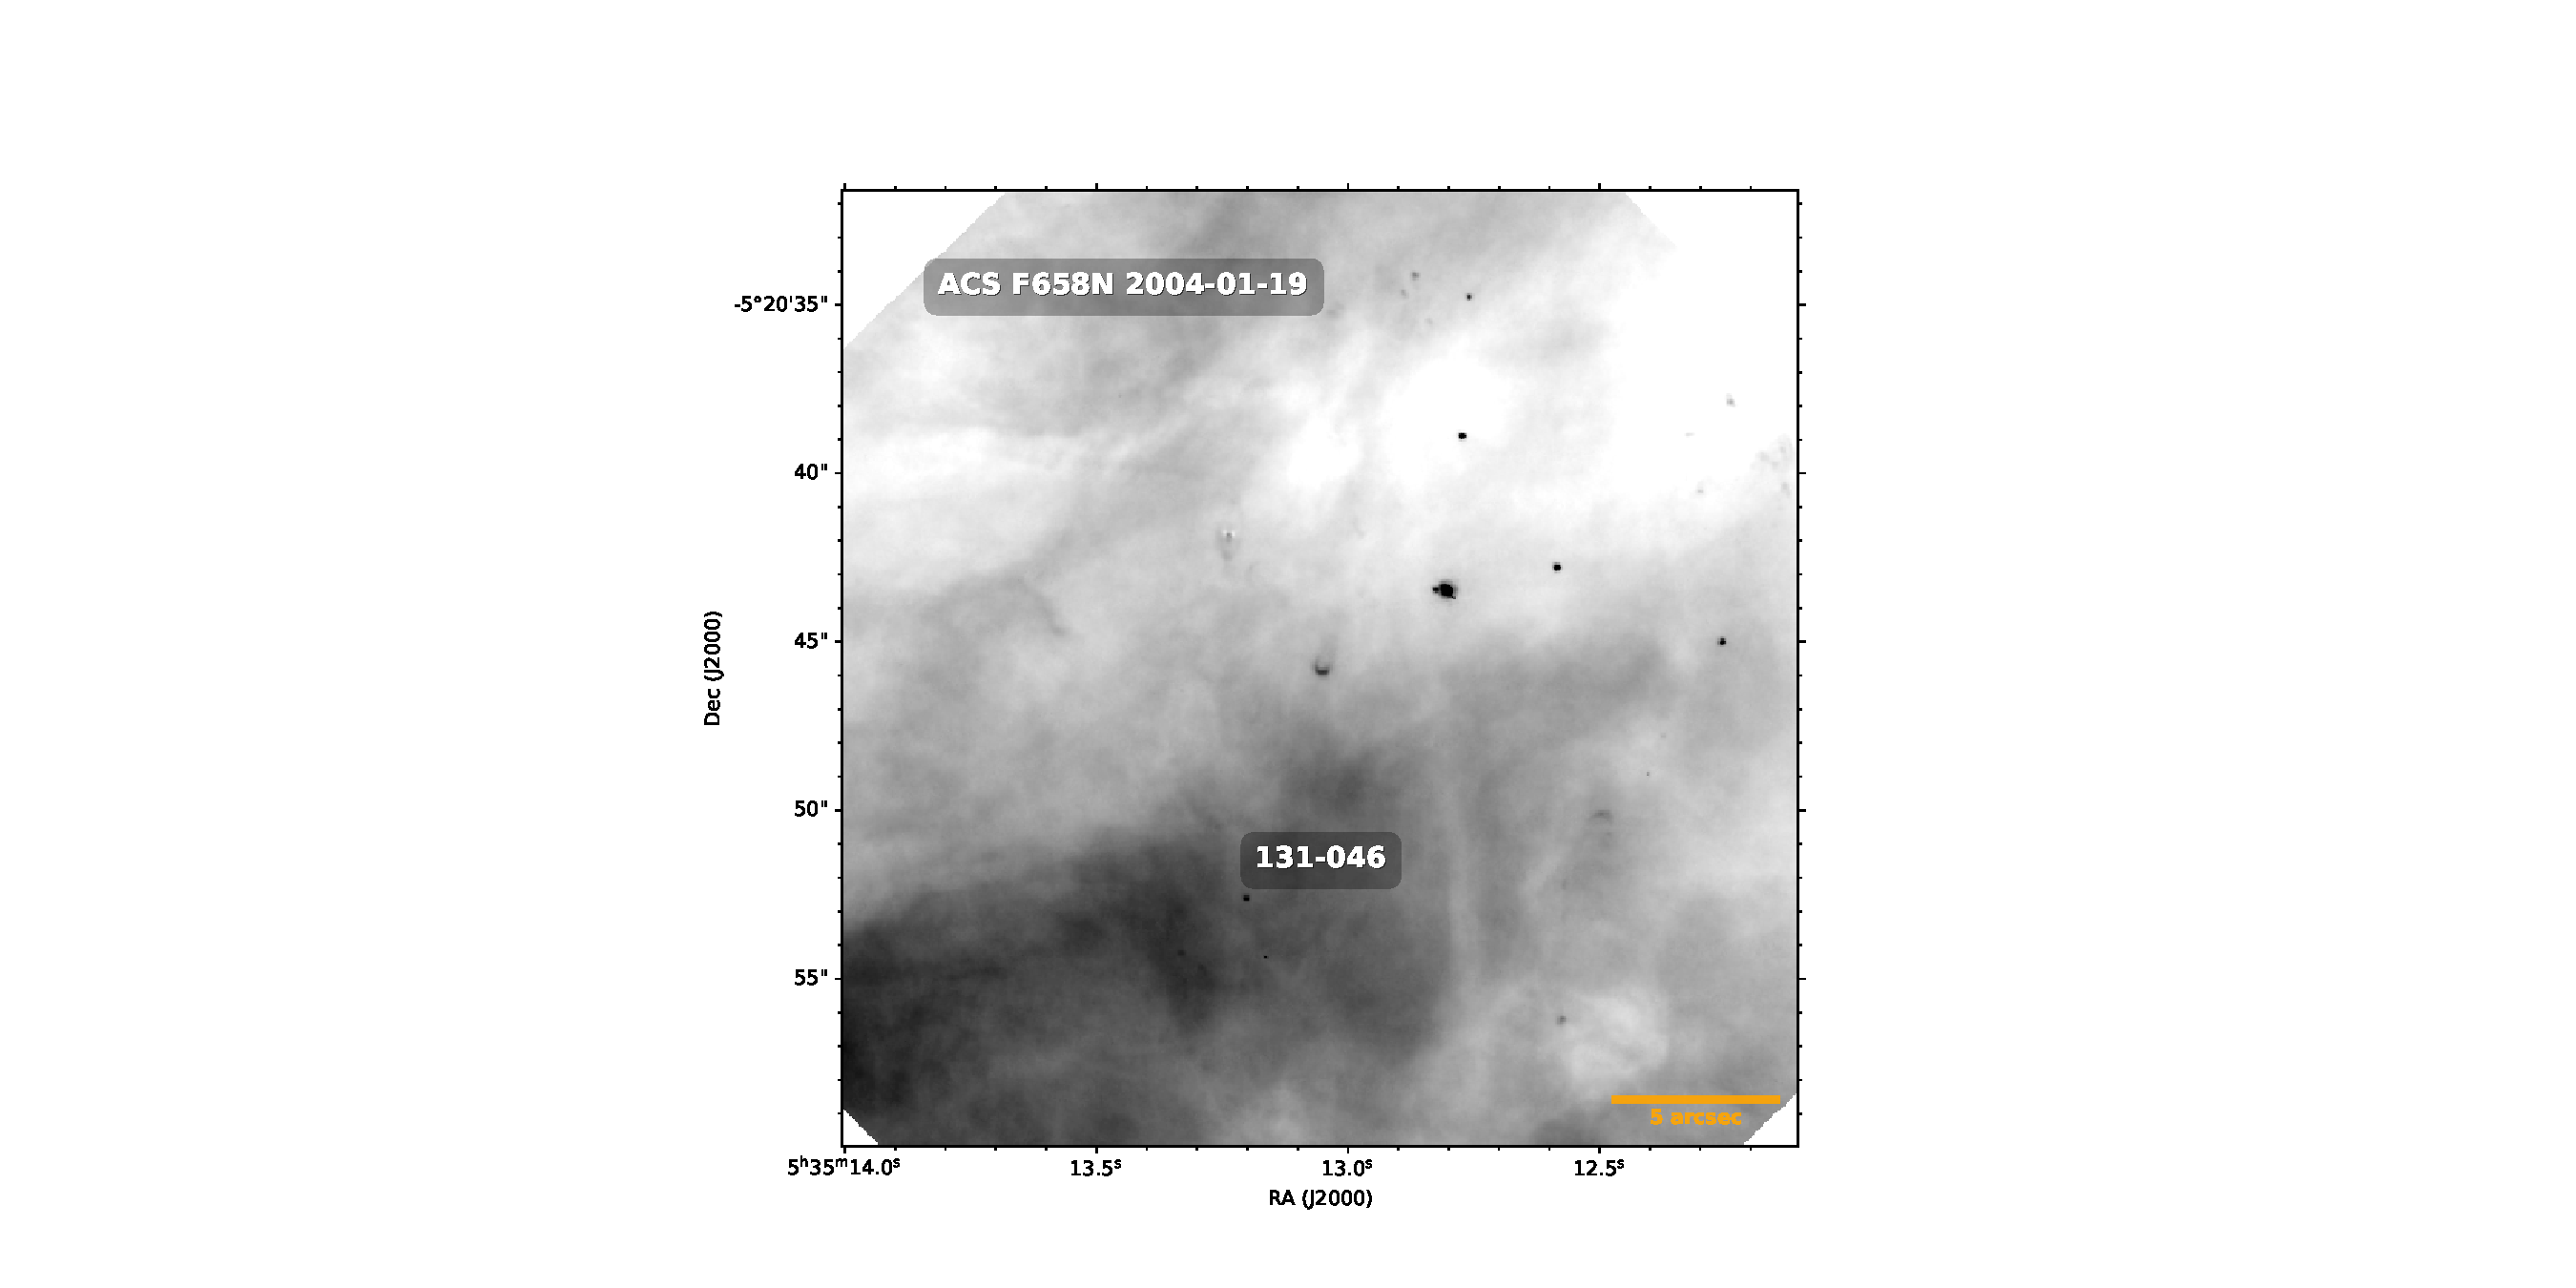
\includegraphics[width=0.165\linewidth, trim=350 10 350 40, clip]{131-046-Bally_02-images-simple} & 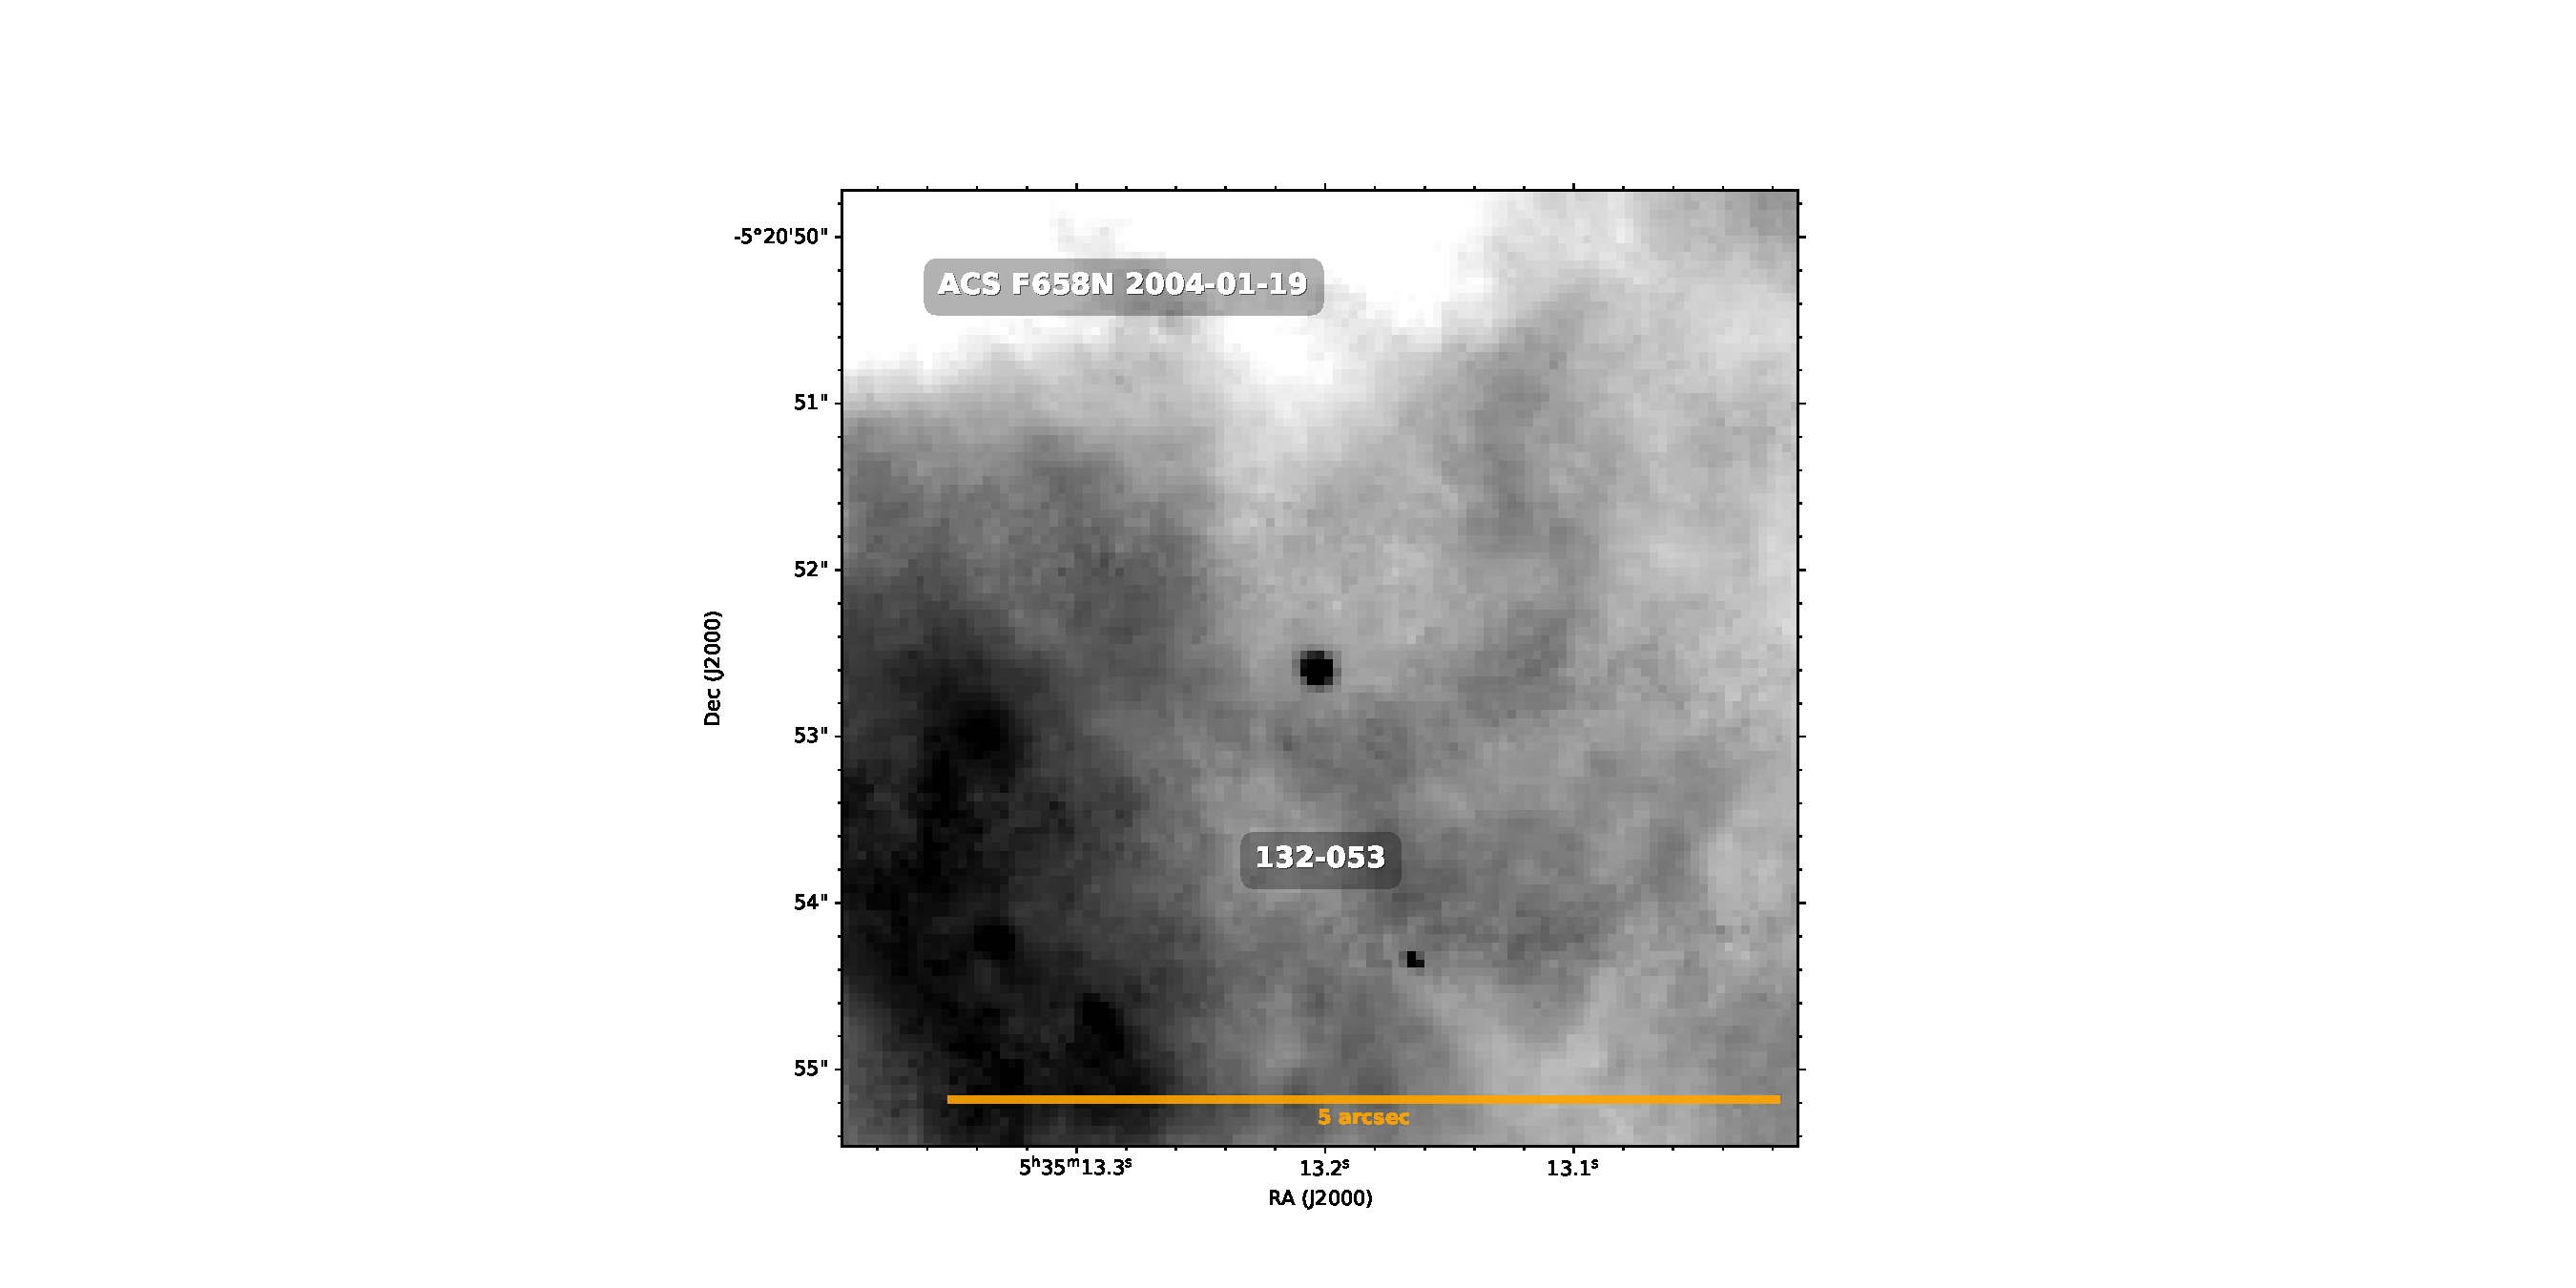
\includegraphics[width=0.165\linewidth, trim=350 10 350 40, clip]{132-053-Bally_02-images-simple} \\
    \raiselabel{(\textit{j})} & \raiselabel{(\textit{k})} & \raiselabel{(\textit{l})} \\
  \end{tabular}
  \caption{Stationary arc sources in the Ambiguous objects.}
  \label{fig:stamps-*P}
\end{figure*}
